% !TEX root = /Users/Gela/Desktop/Thesis_latex/thesis.tex


\section{Flowchart investigation}
Two different setups for a comparing system to the current system were investigated, section \ref{Flowchart}, and System 2 were chosen to be the comparing system. Both Systems were considered fulfilling most of the requirements, section \ref{framing}, for an updated version. \\

In order to choose one comparing system benefits and disadvantages with the two system were investigated. \\

System 1, figure \ref{fig:FlowCInves1}, is considered capable of creating a high pressure drop over the membrane. The hypothesis is also that it is capable of creating the biggest pressure drop with the least amount of energy needed. A disadvantage is considered  that implementing a pump in the purified water path will increase the risk that the pump may release particles into purified water which is, from a patient safety perspective, a high risk factor. \\

System 2, figure \ref{fig:Sys2}, is considered capable of creating a high pressure drop over the membrane. It is also capable of controlling the recovery factor which, due to theory increases the membrane life time and performance. It might also be capable of minimize the salt concentration close to membrane surface area if increasing recirculation flow, e.g, create turbulence close to the membrane surface. \\


The two comparing systems were set to:\\
\begin{figure}[h]
\centering
\begin{minipage}{.5\textwidth}
    \centering
    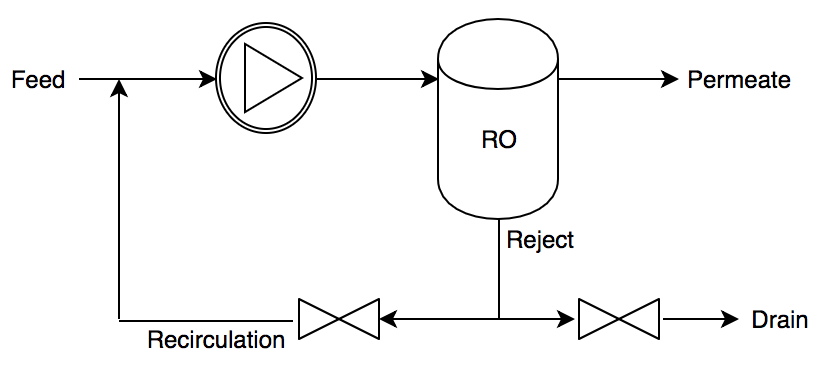
\includegraphics[width=0.8\textwidth]{Sys1}
    \caption{Current System}
    \label{fig:System1}
\end{minipage}%
\begin{minipage}{.5\textwidth}
  \centering
  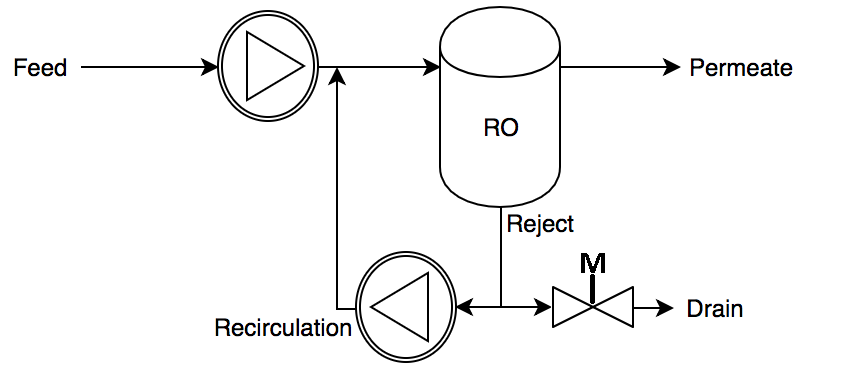
\includegraphics[width=.8\linewidth]{Sys2}
  \caption{System 2}
  \label{fig:System2}
\end{minipage}
\end{figure}

\section{Tests}
\subsection{Current system}
Results for the test on the current system, figure \ref{fig:Sys1}:

Room temperature:




\begin{figure}[H]
    \centering
    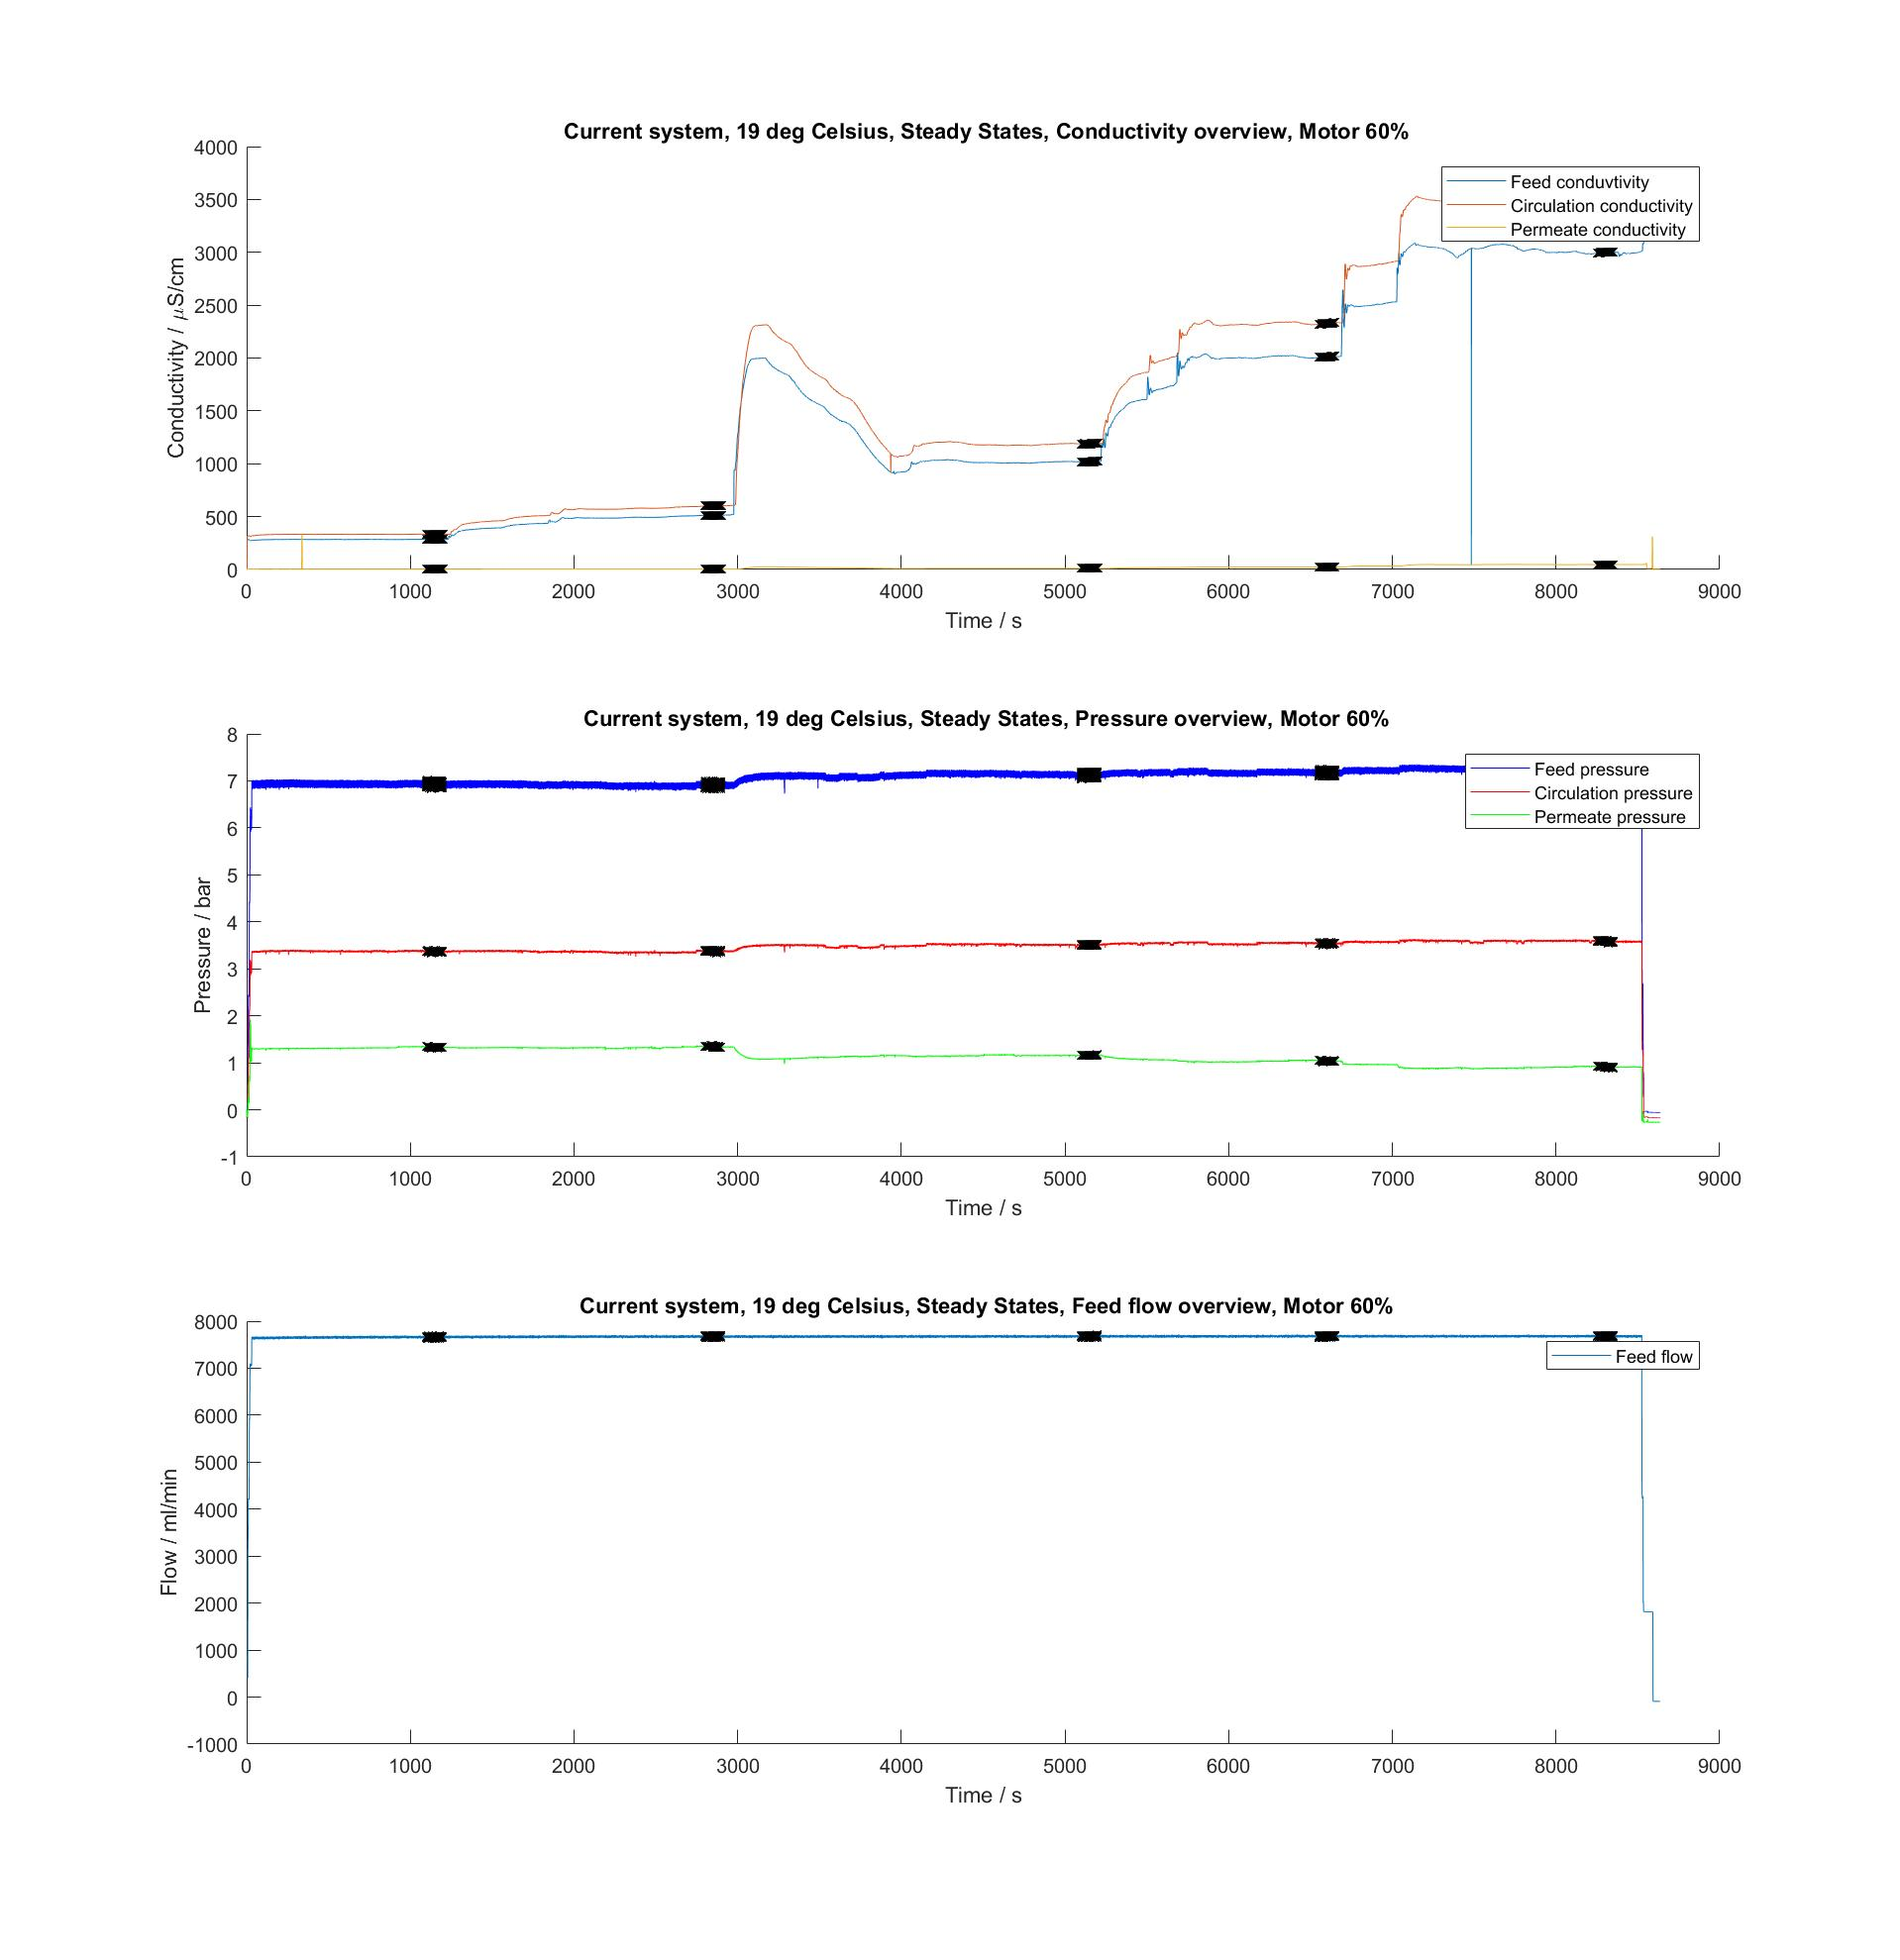
\includegraphics[width=1.1\textwidth]{overview20_60}
    \caption{Connections Pressure sensors}
    \label{fig:PressConn}
\end{figure}


\begin{figure}[H]
    \centering
    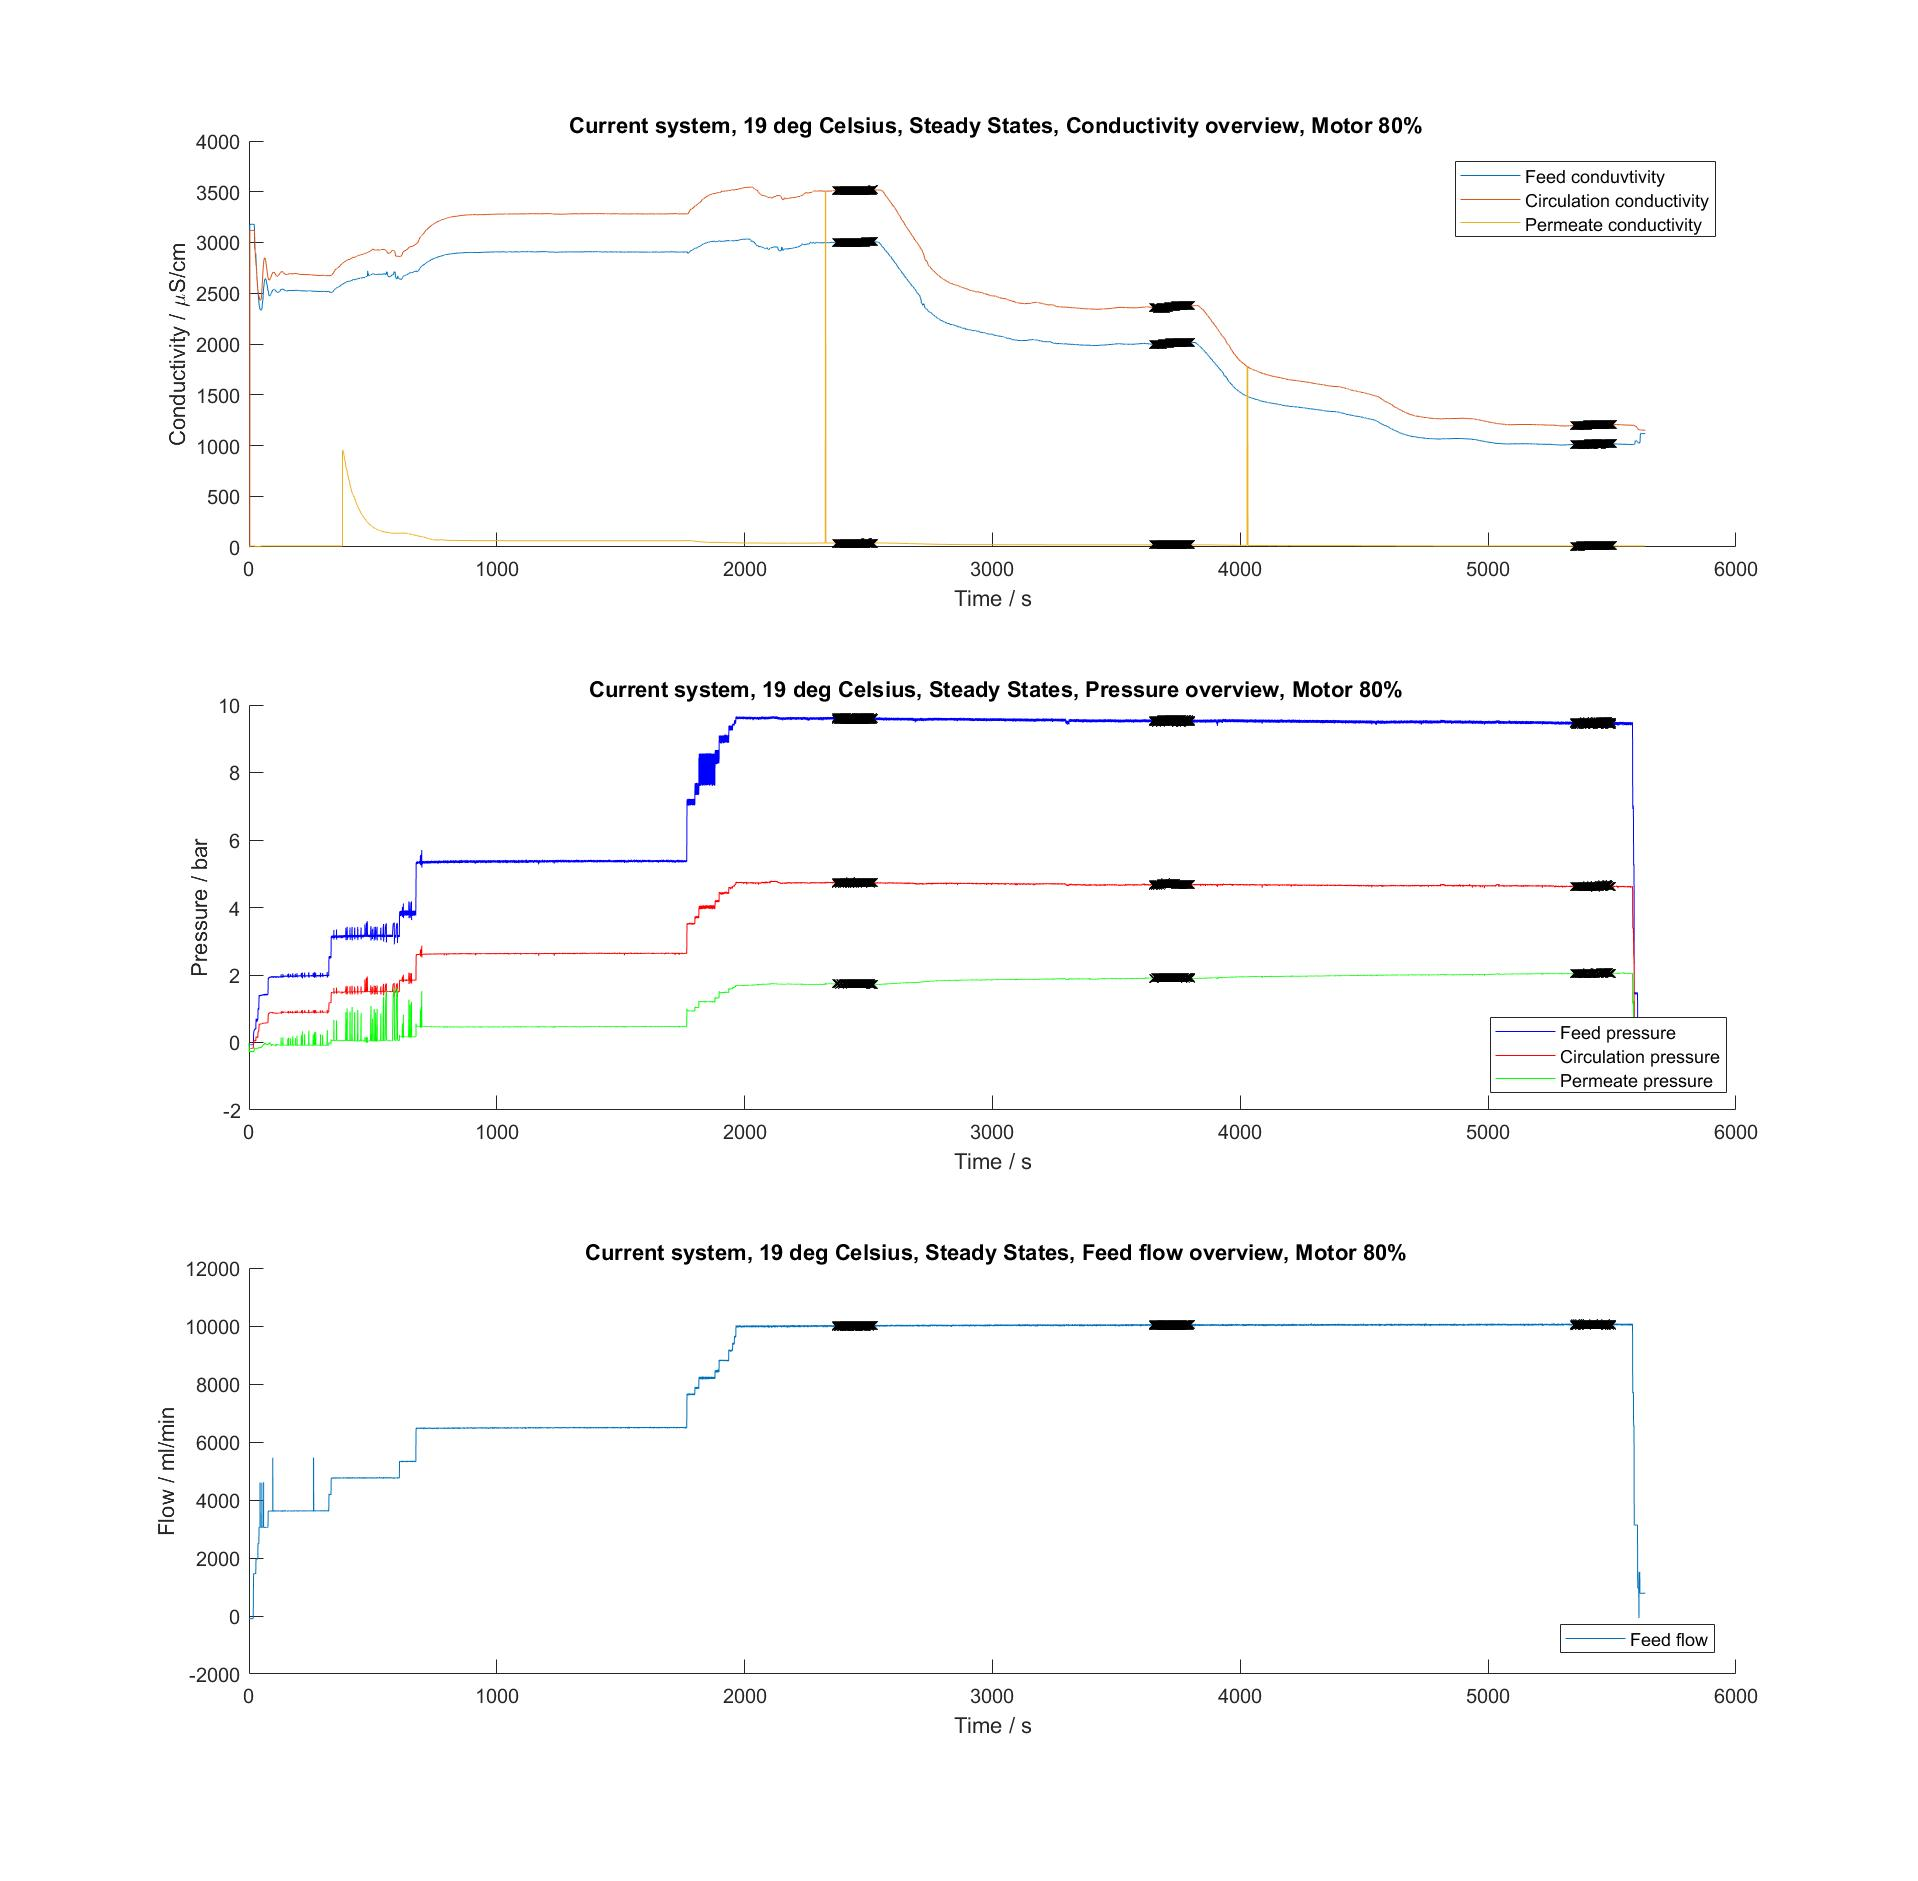
\includegraphics[width=1.1\textwidth]{overview20_80}
    \caption{Connections Pressure sensors}
    \label{fig:PressConn}
\end{figure}

\begin{figure}[H]
    \centering
    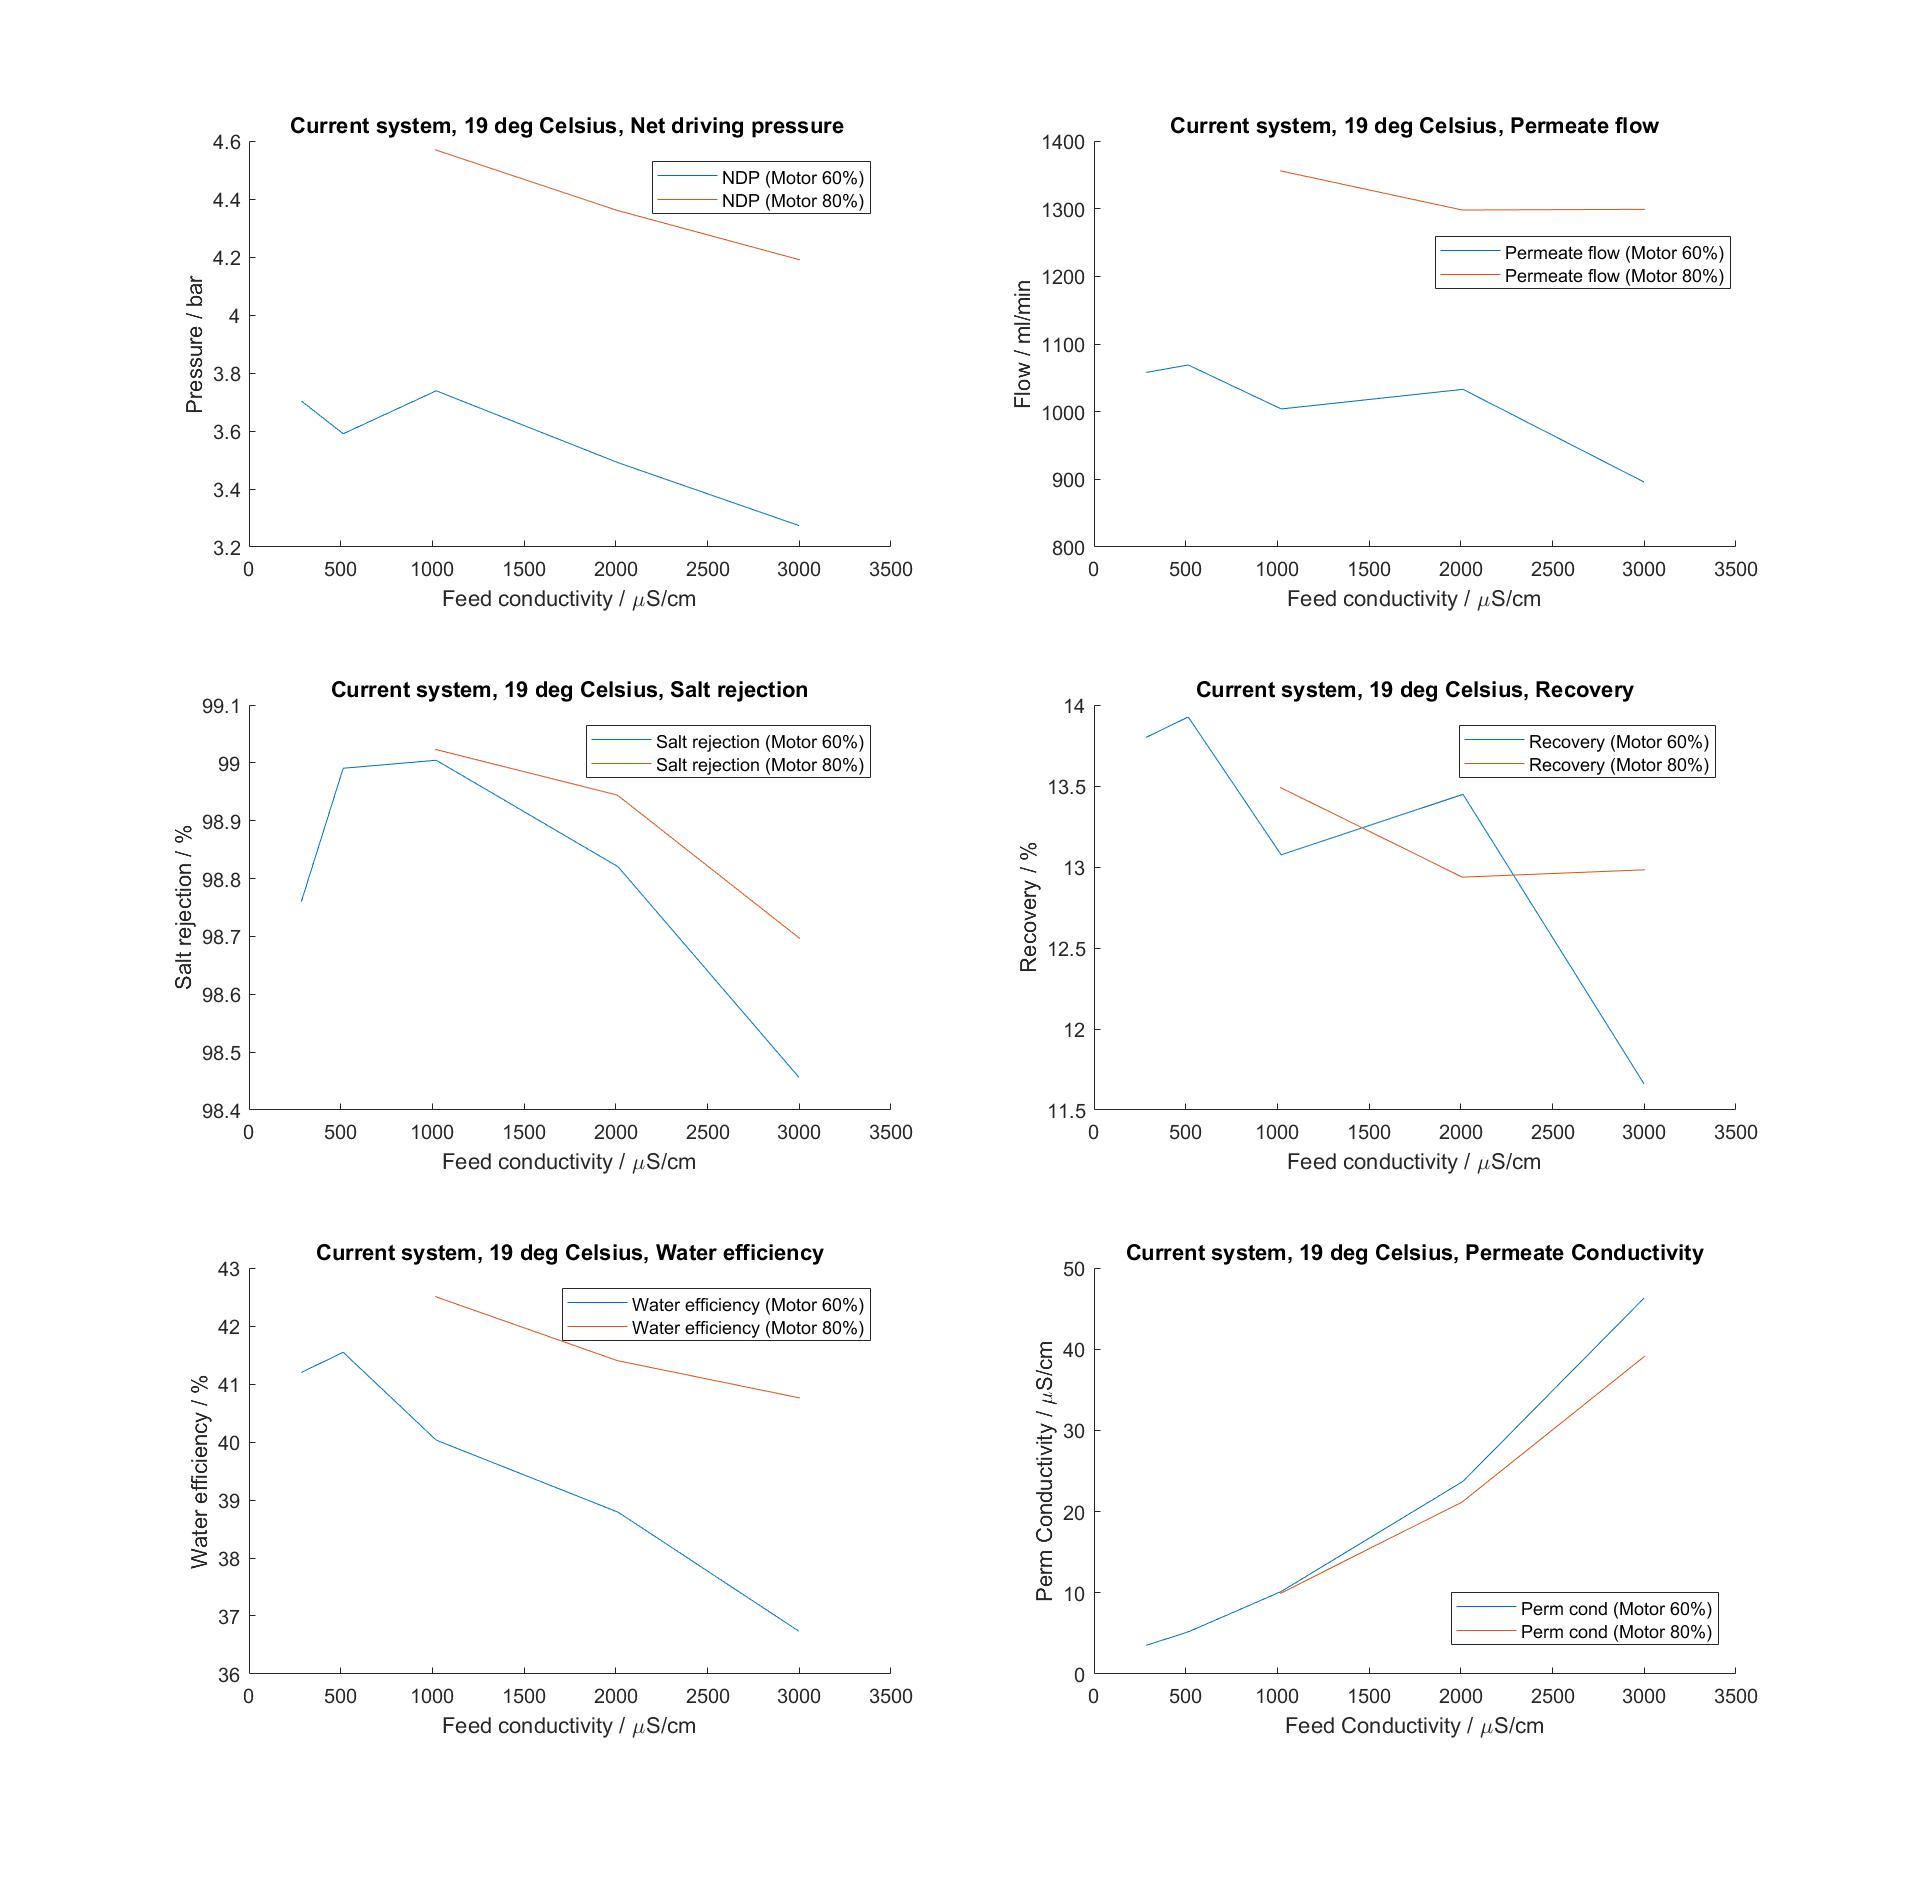
\includegraphics[width=1.1\textwidth]{Key20}
    \caption{Connections Pressure sensors}
    \label{fig:PressConn}
\end{figure}

short explanation of tests.

Tests conducted at 30 deg C.

\begin{figure}[H]
    \centering
    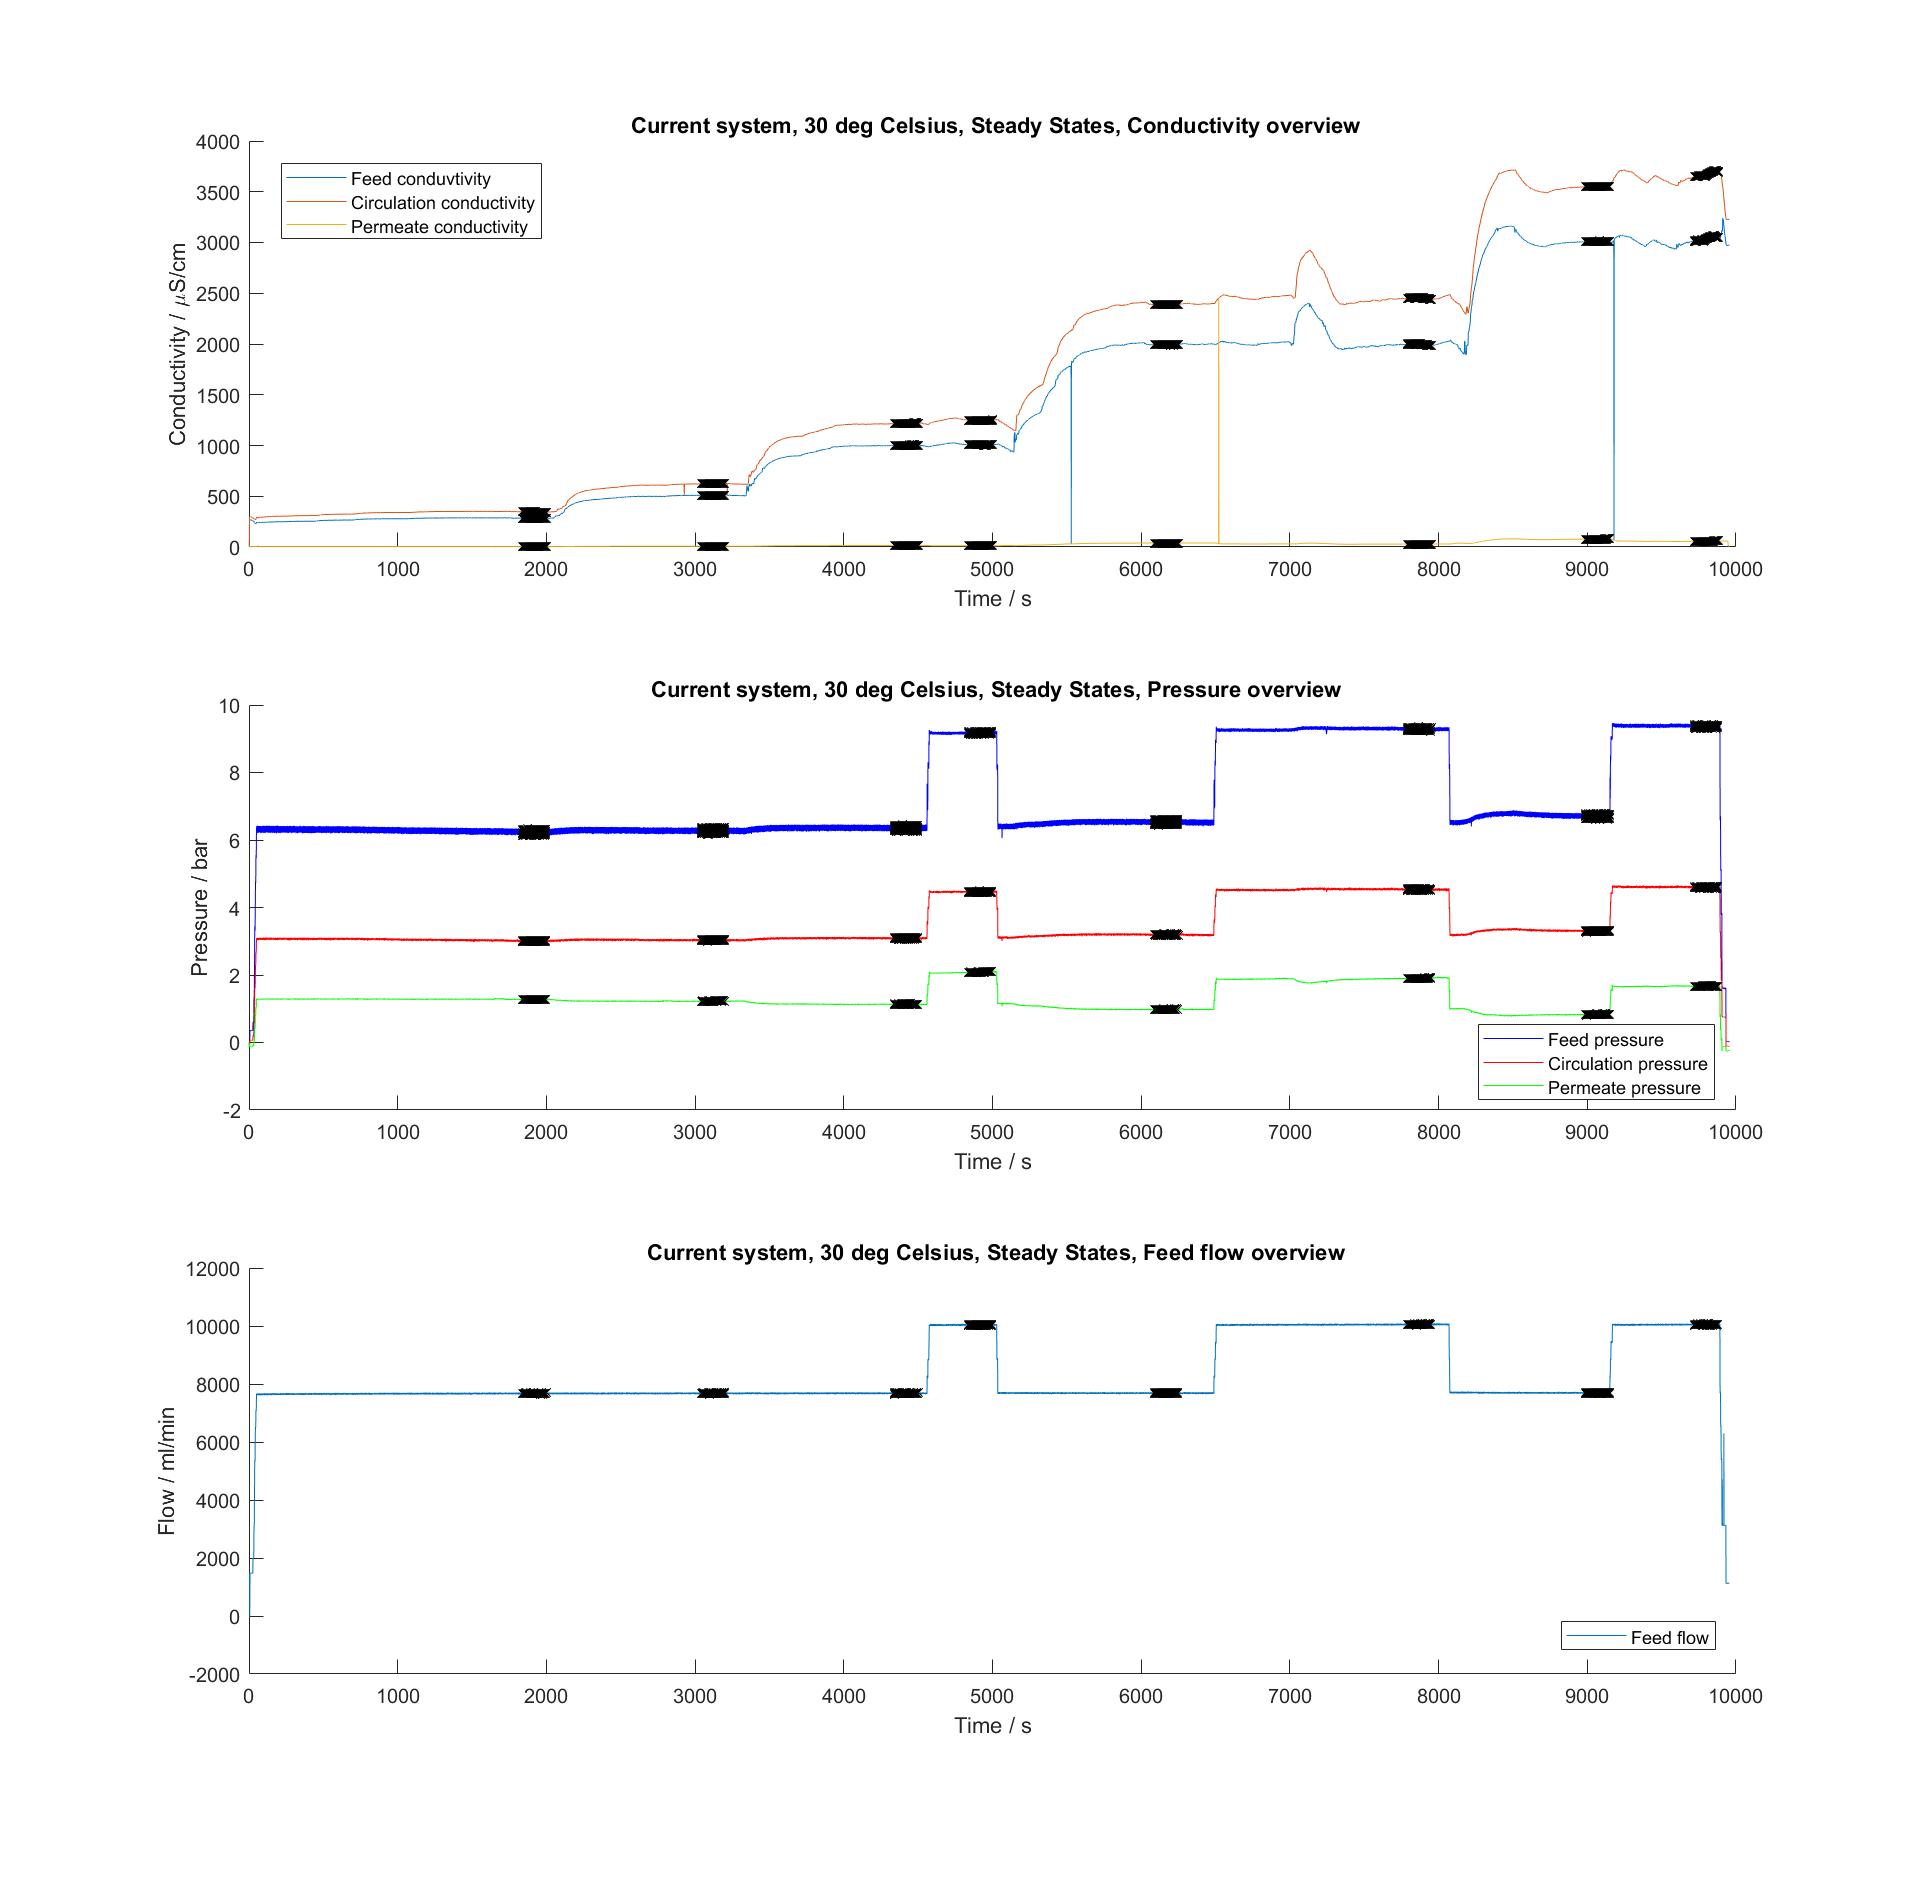
\includegraphics[width=1.1\textwidth]{overview30}
    \caption{Connections Pressure sensors}
    \label{fig:PressConn}
\end{figure}

\begin{figure}[H]
    \centering
    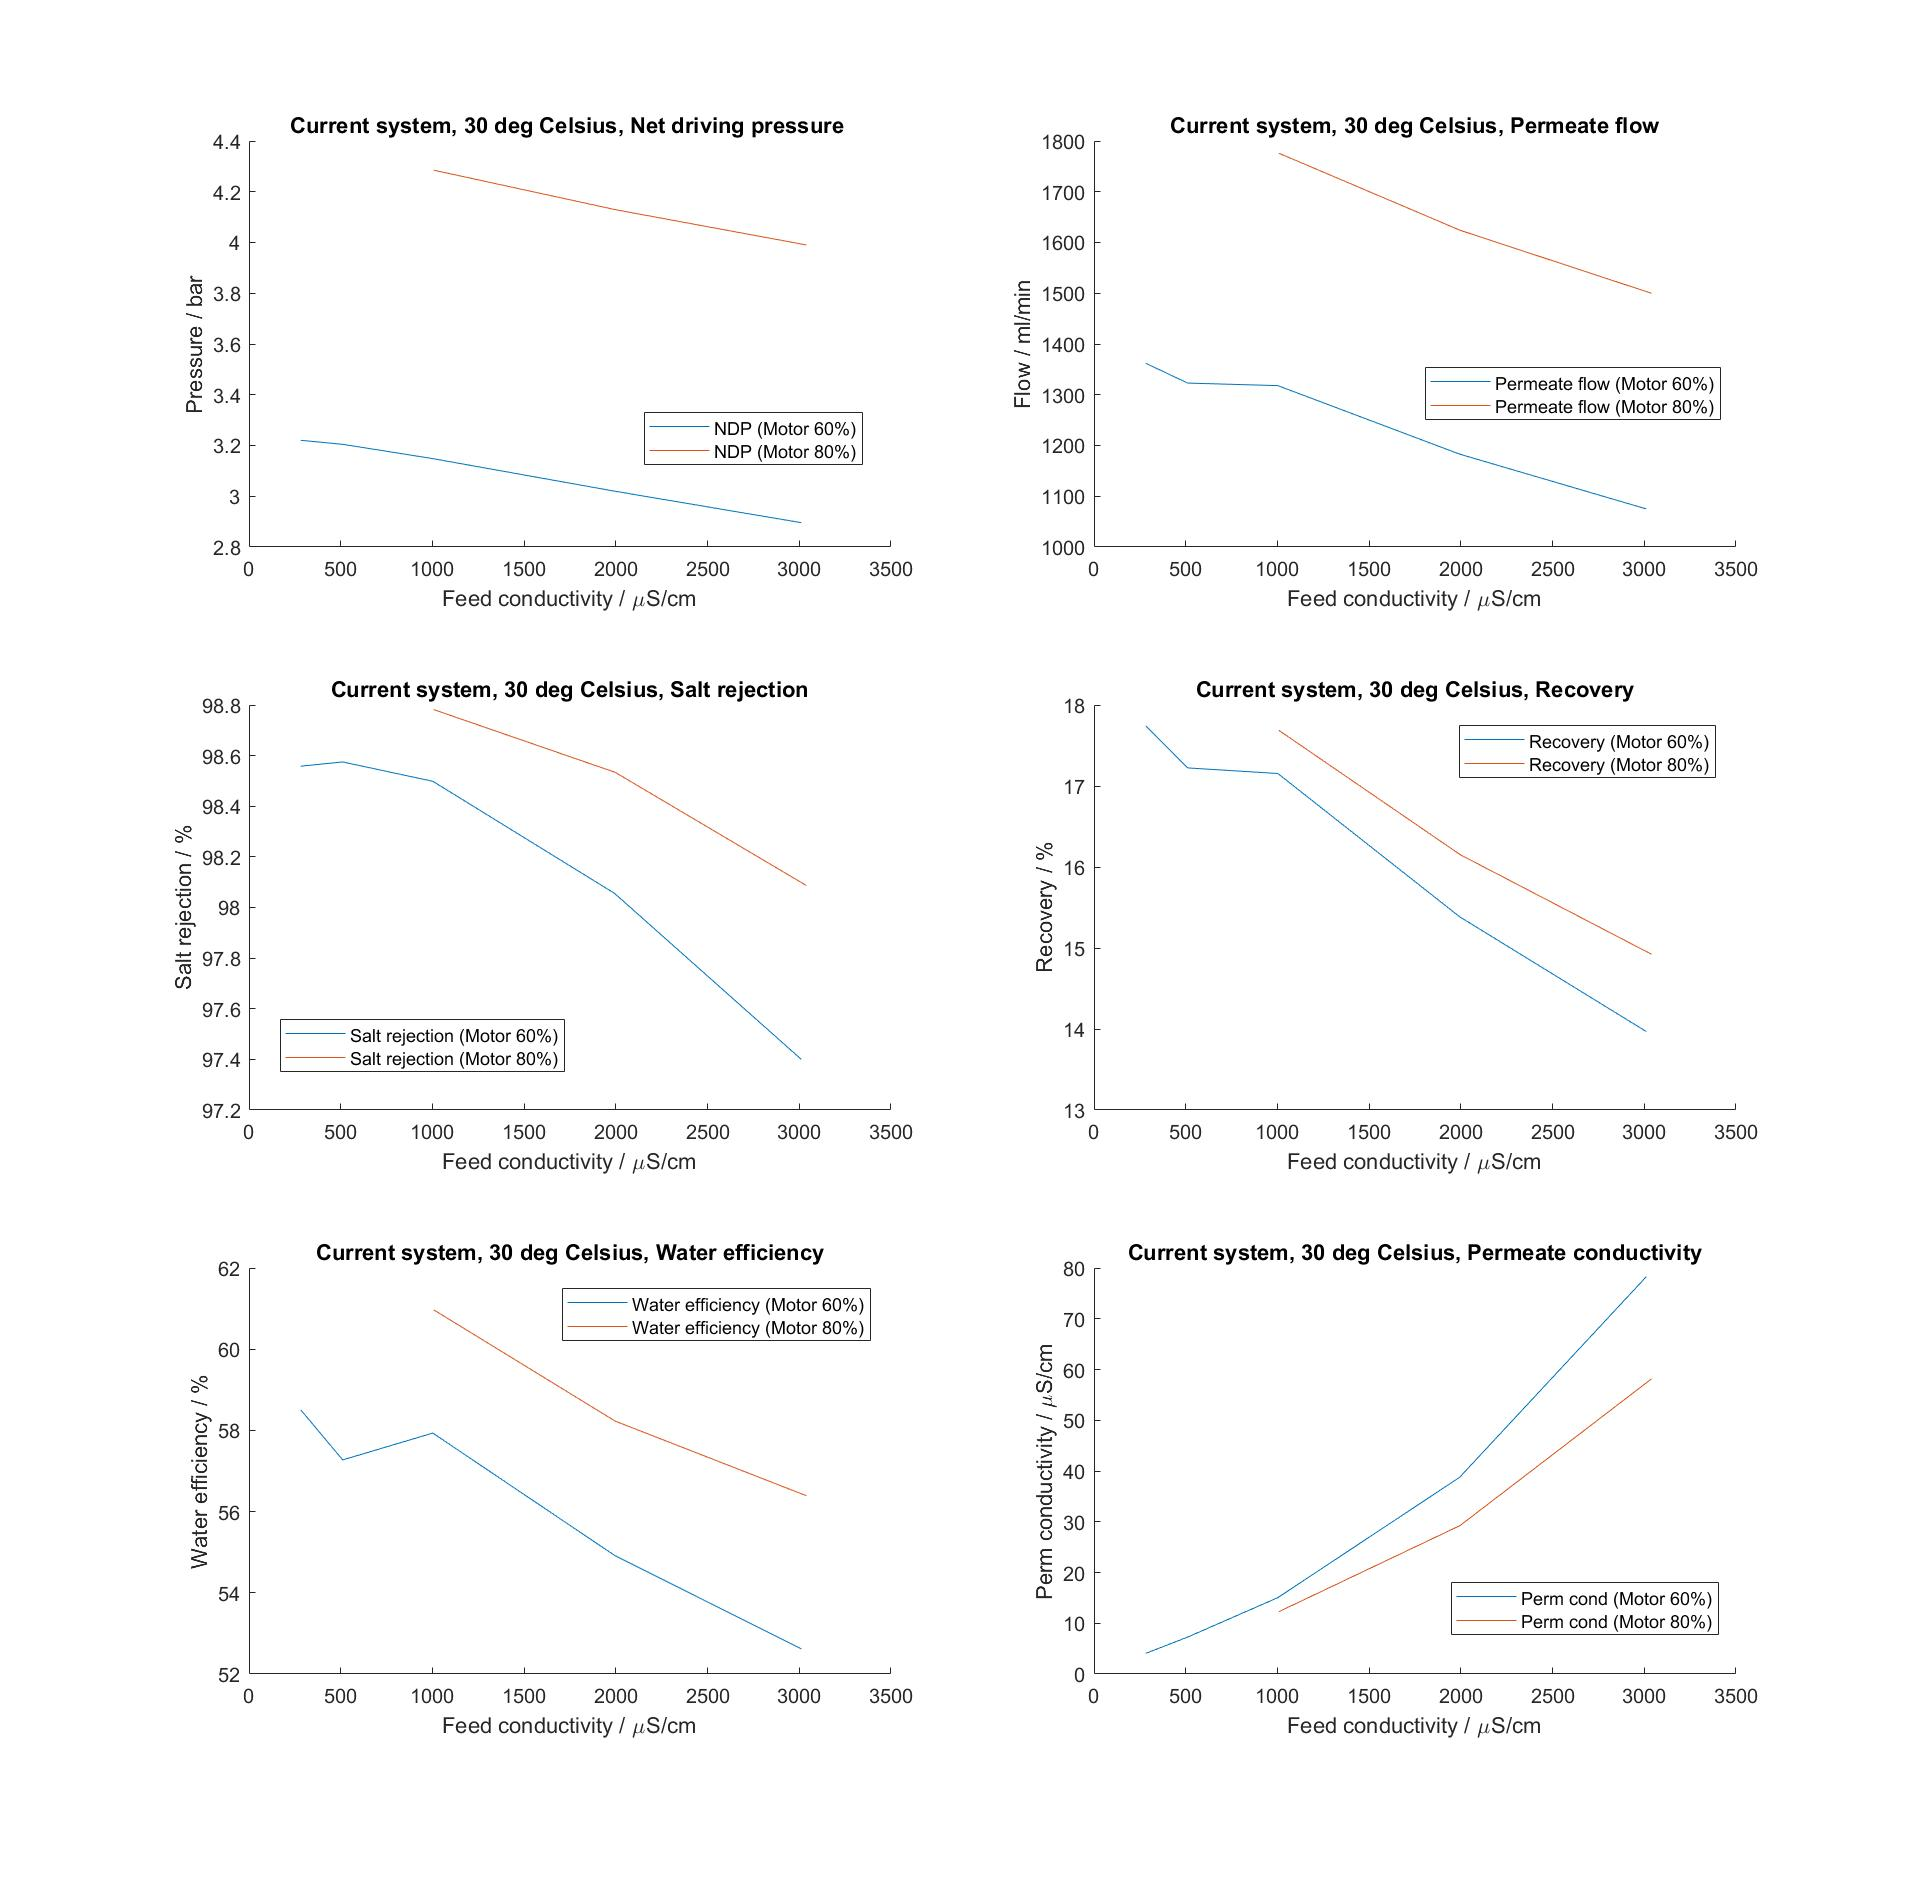
\includegraphics[width=1.1\textwidth]{Key30}
    \caption{Connections Pressure sensors}
    \label{fig:PressConn}
\end{figure}

Tests conducted at 40 deg C.''

\begin{figure}[H]
    \centering
    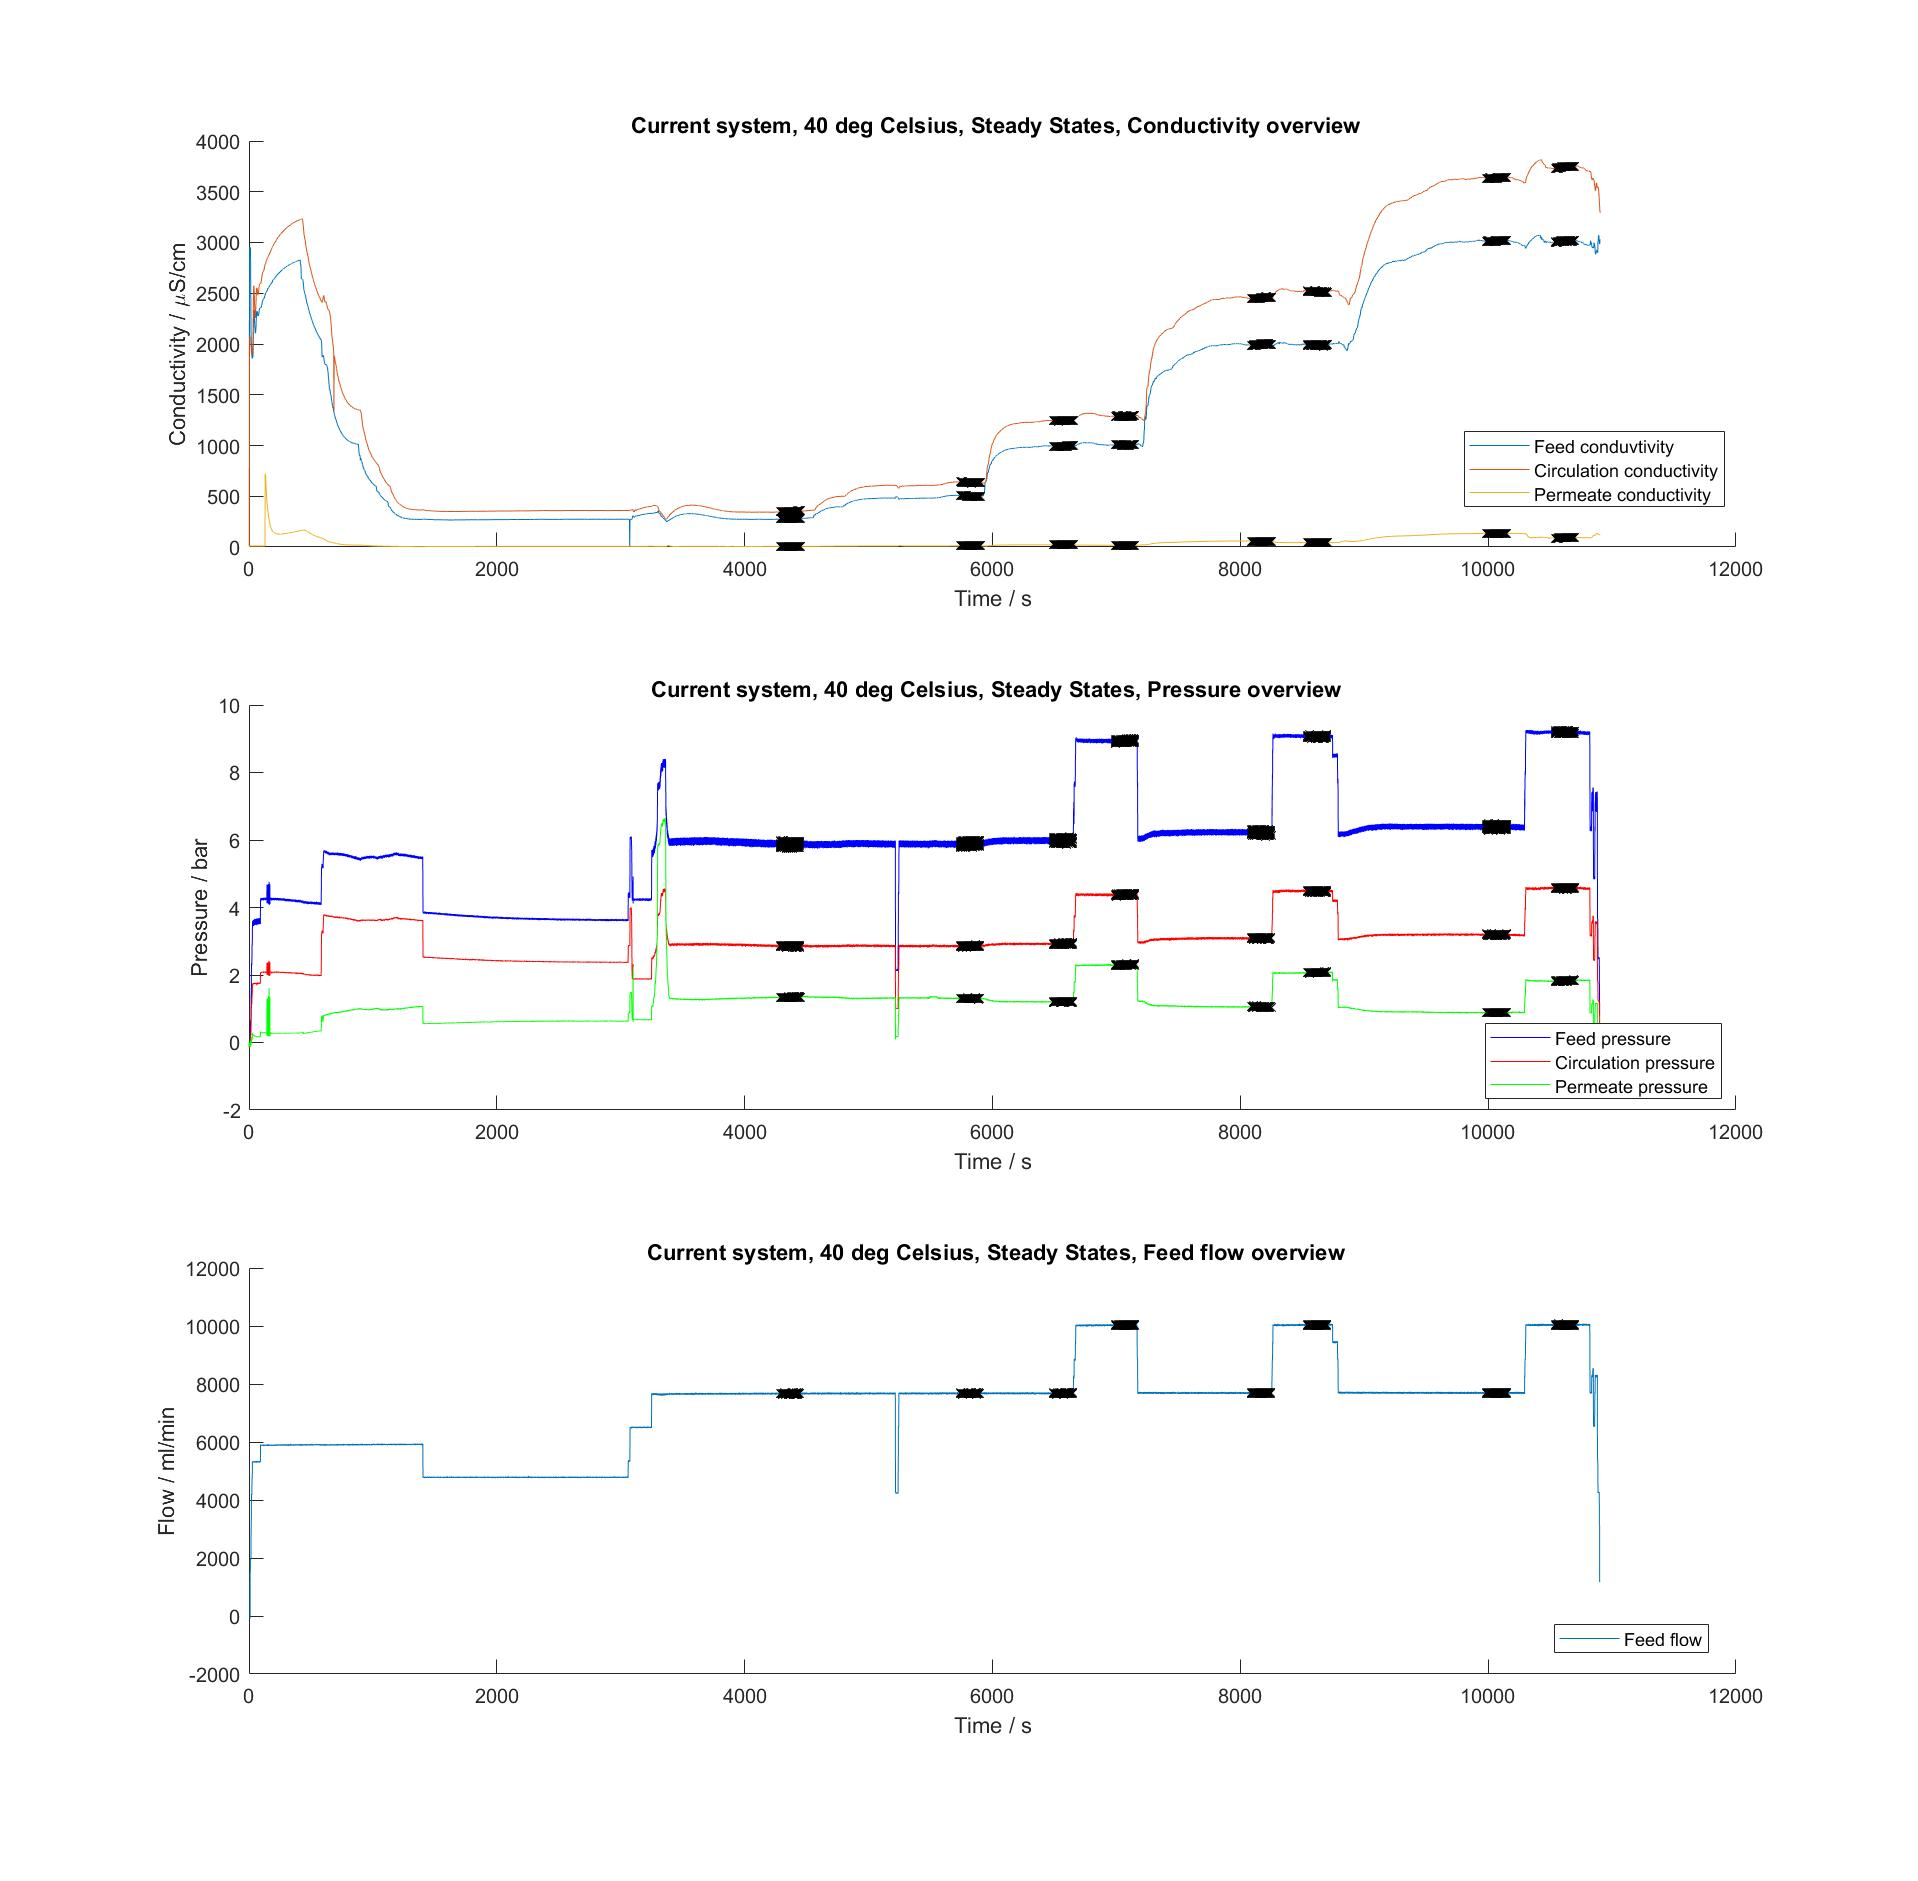
\includegraphics[width=1.1\textwidth]{overview40}
    \caption{Connections Pressure sensors}
    \label{fig:PressConn}
\end{figure}

\begin{figure}[H]
    \centering
    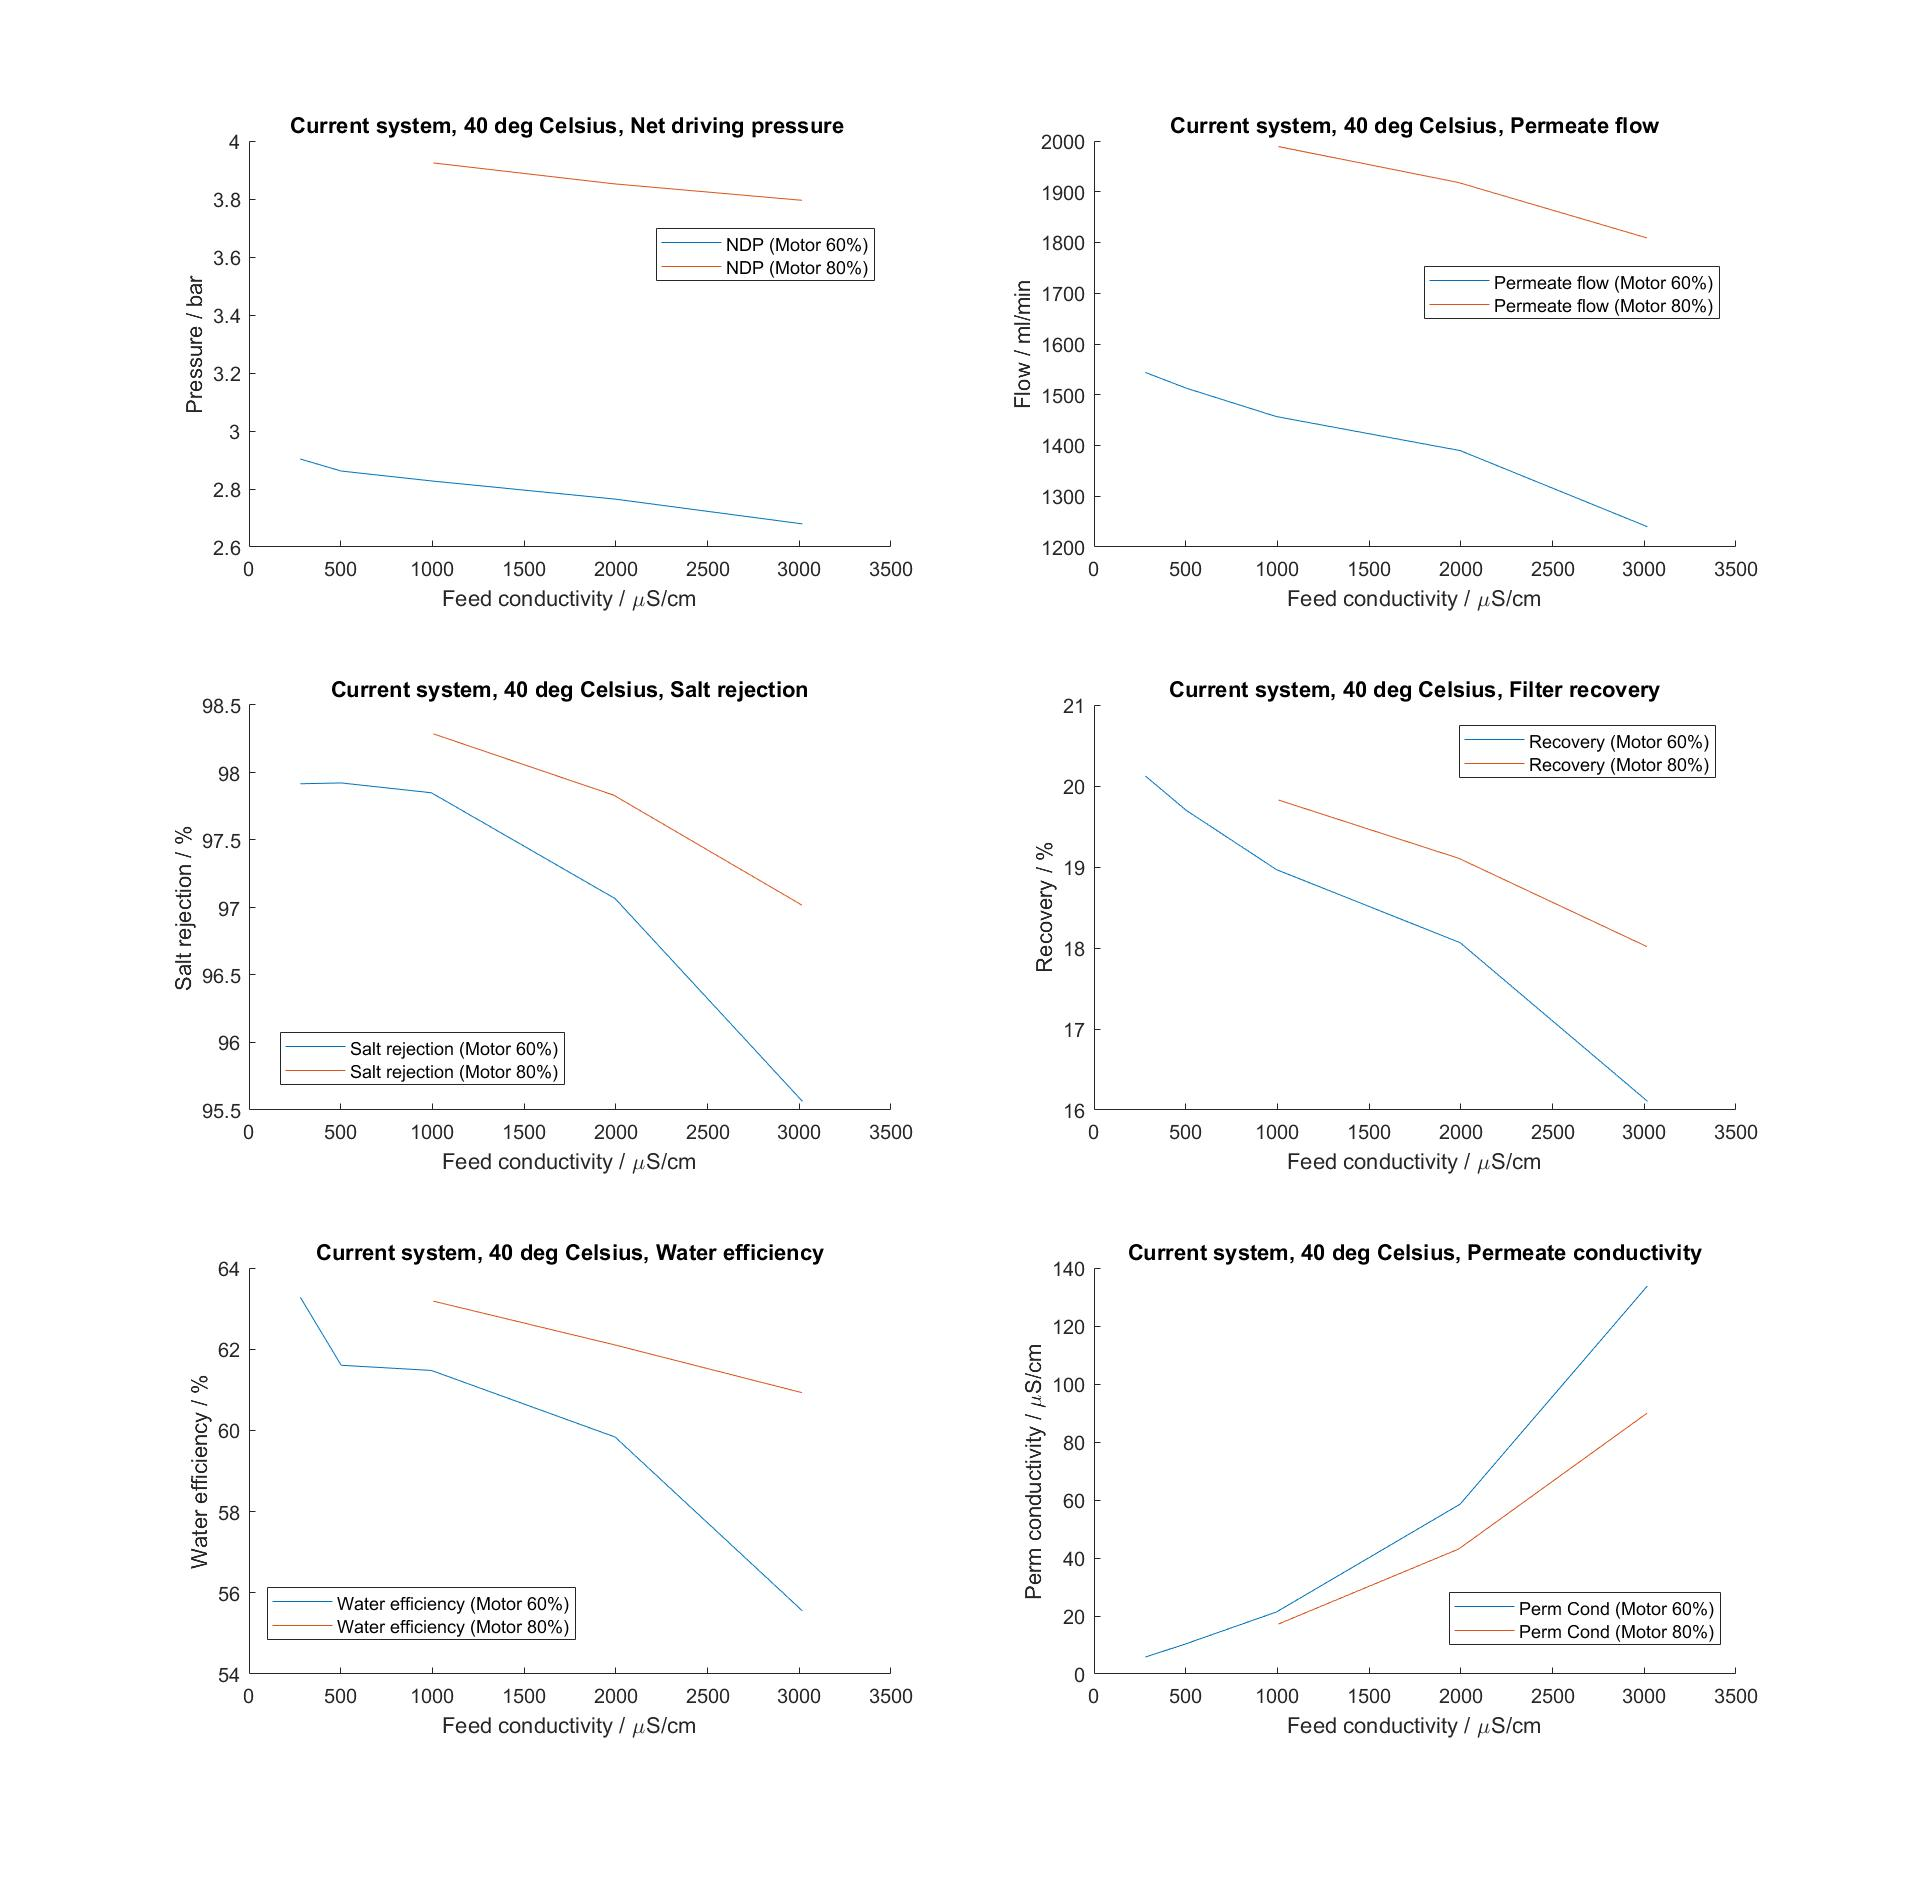
\includegraphics[width=1.1\textwidth]{Key40}
    \caption{Connections Pressure sensors}
    \label{fig:PressConn}
\end{figure}

\begin{figure}[H]
    \centering
    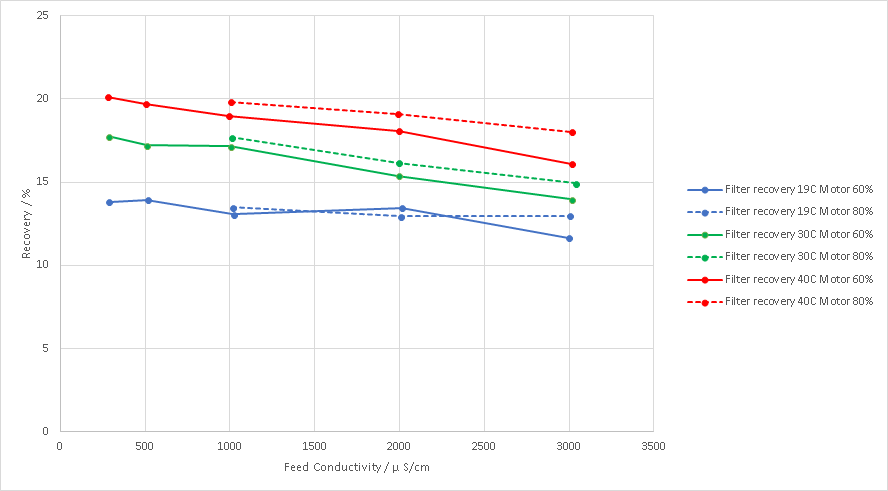
\includegraphics[width=1.1\textwidth]{Recovery}
    \caption{Connections Pressure sensors}
    \label{fig:PressConn}
\end{figure}

\begin{figure}[H]
    \centering
    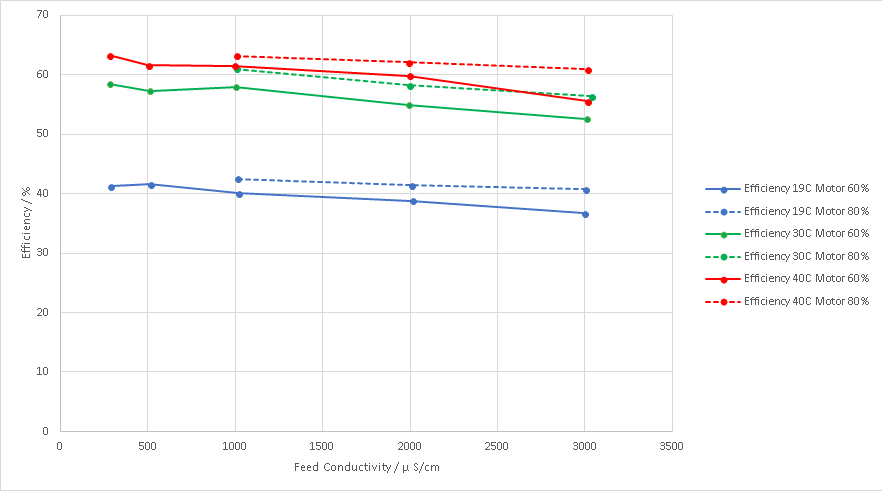
\includegraphics[width=1.1\textwidth]{Efficiency}
    \caption{Connections Pressure sensors}
    \label{fig:PressConn}
\end{figure}

\begin{figure}[H]
    \centering
    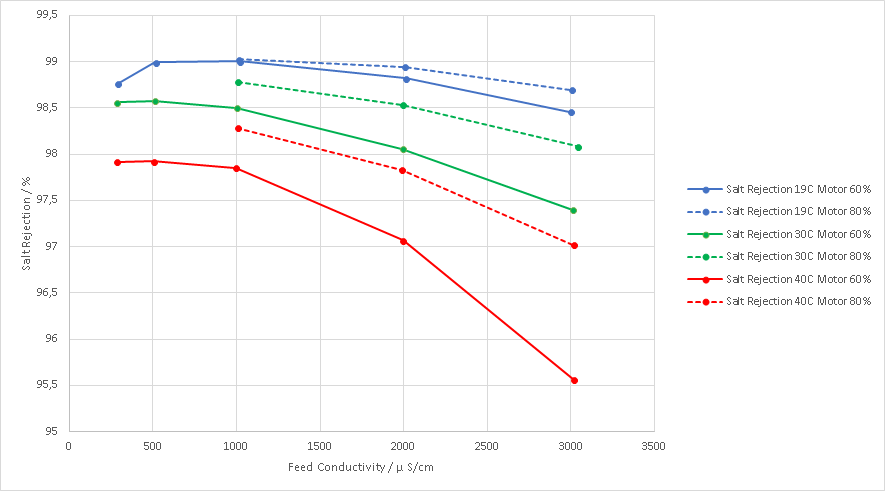
\includegraphics[width=1.1\textwidth]{SaltRejection}
    \caption{Connections Pressure sensors}
    \label{fig:PressConn}
\end{figure}

\begin{figure}[H]
    \centering
    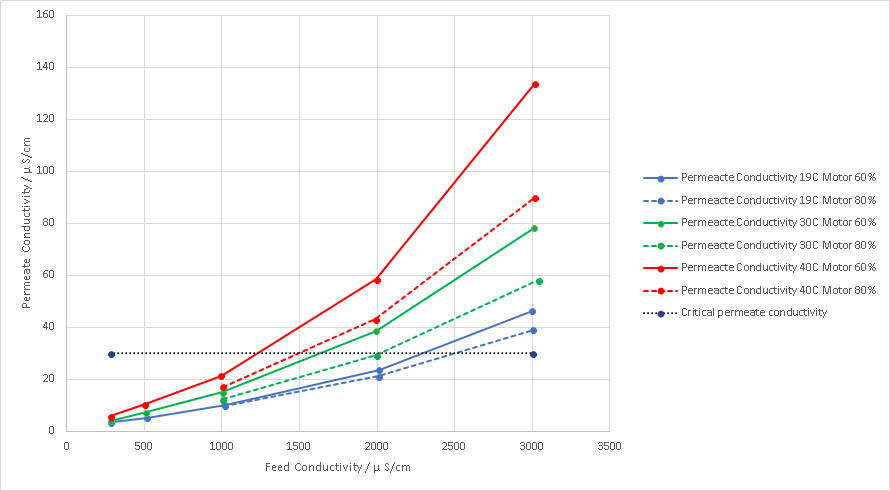
\includegraphics[width=1.1\textwidth]{PermCond}
    \caption{Connections Pressure sensors}
    \label{fig:PressConn}
\end{figure}

\begin{figure}[H]
    \centering
    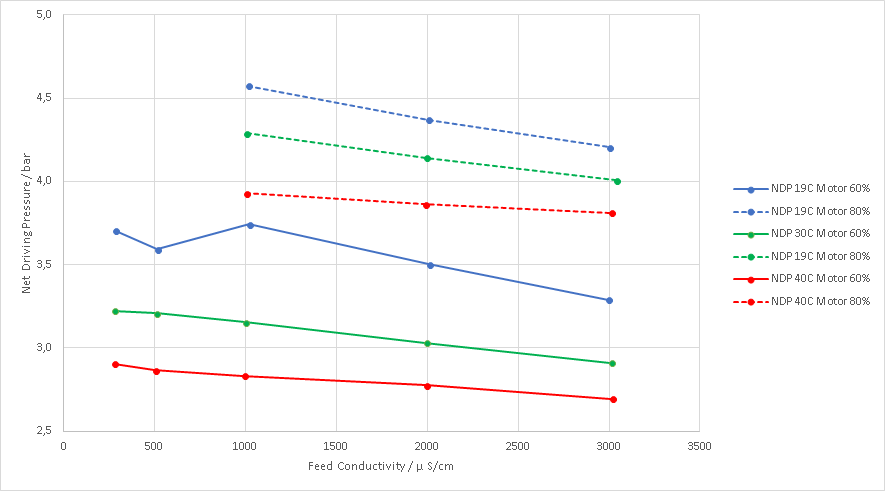
\includegraphics[width=1.1\textwidth]{NDP}
    \caption{Connections Pressure sensors}
    \label{fig:PressConn}
\end{figure}

\begin{figure}[H]
    \centering
    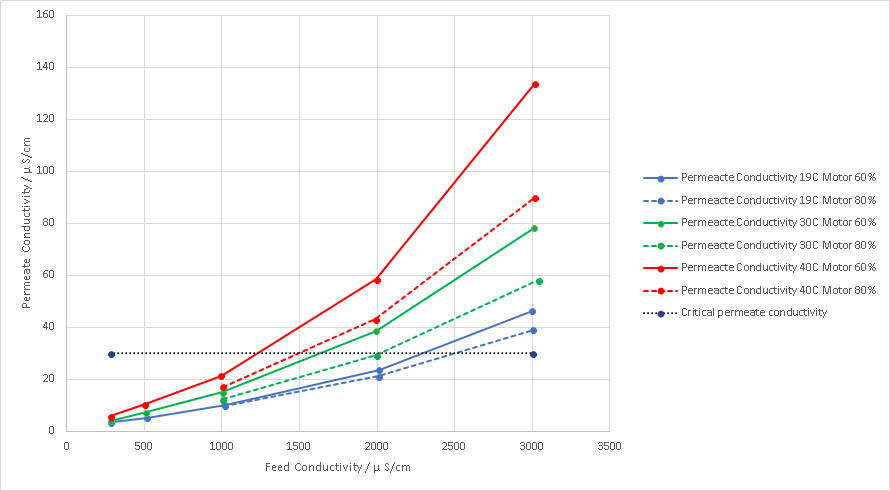
\includegraphics[width=1.1\textwidth]{PermCond}
    \caption{Connections Pressure sensors}
    \label{fig:PressConn}
\end{figure}





\subsection{System 2}

Test: increaed feed pressure

21


\begin{figure}[H]
    \centering
    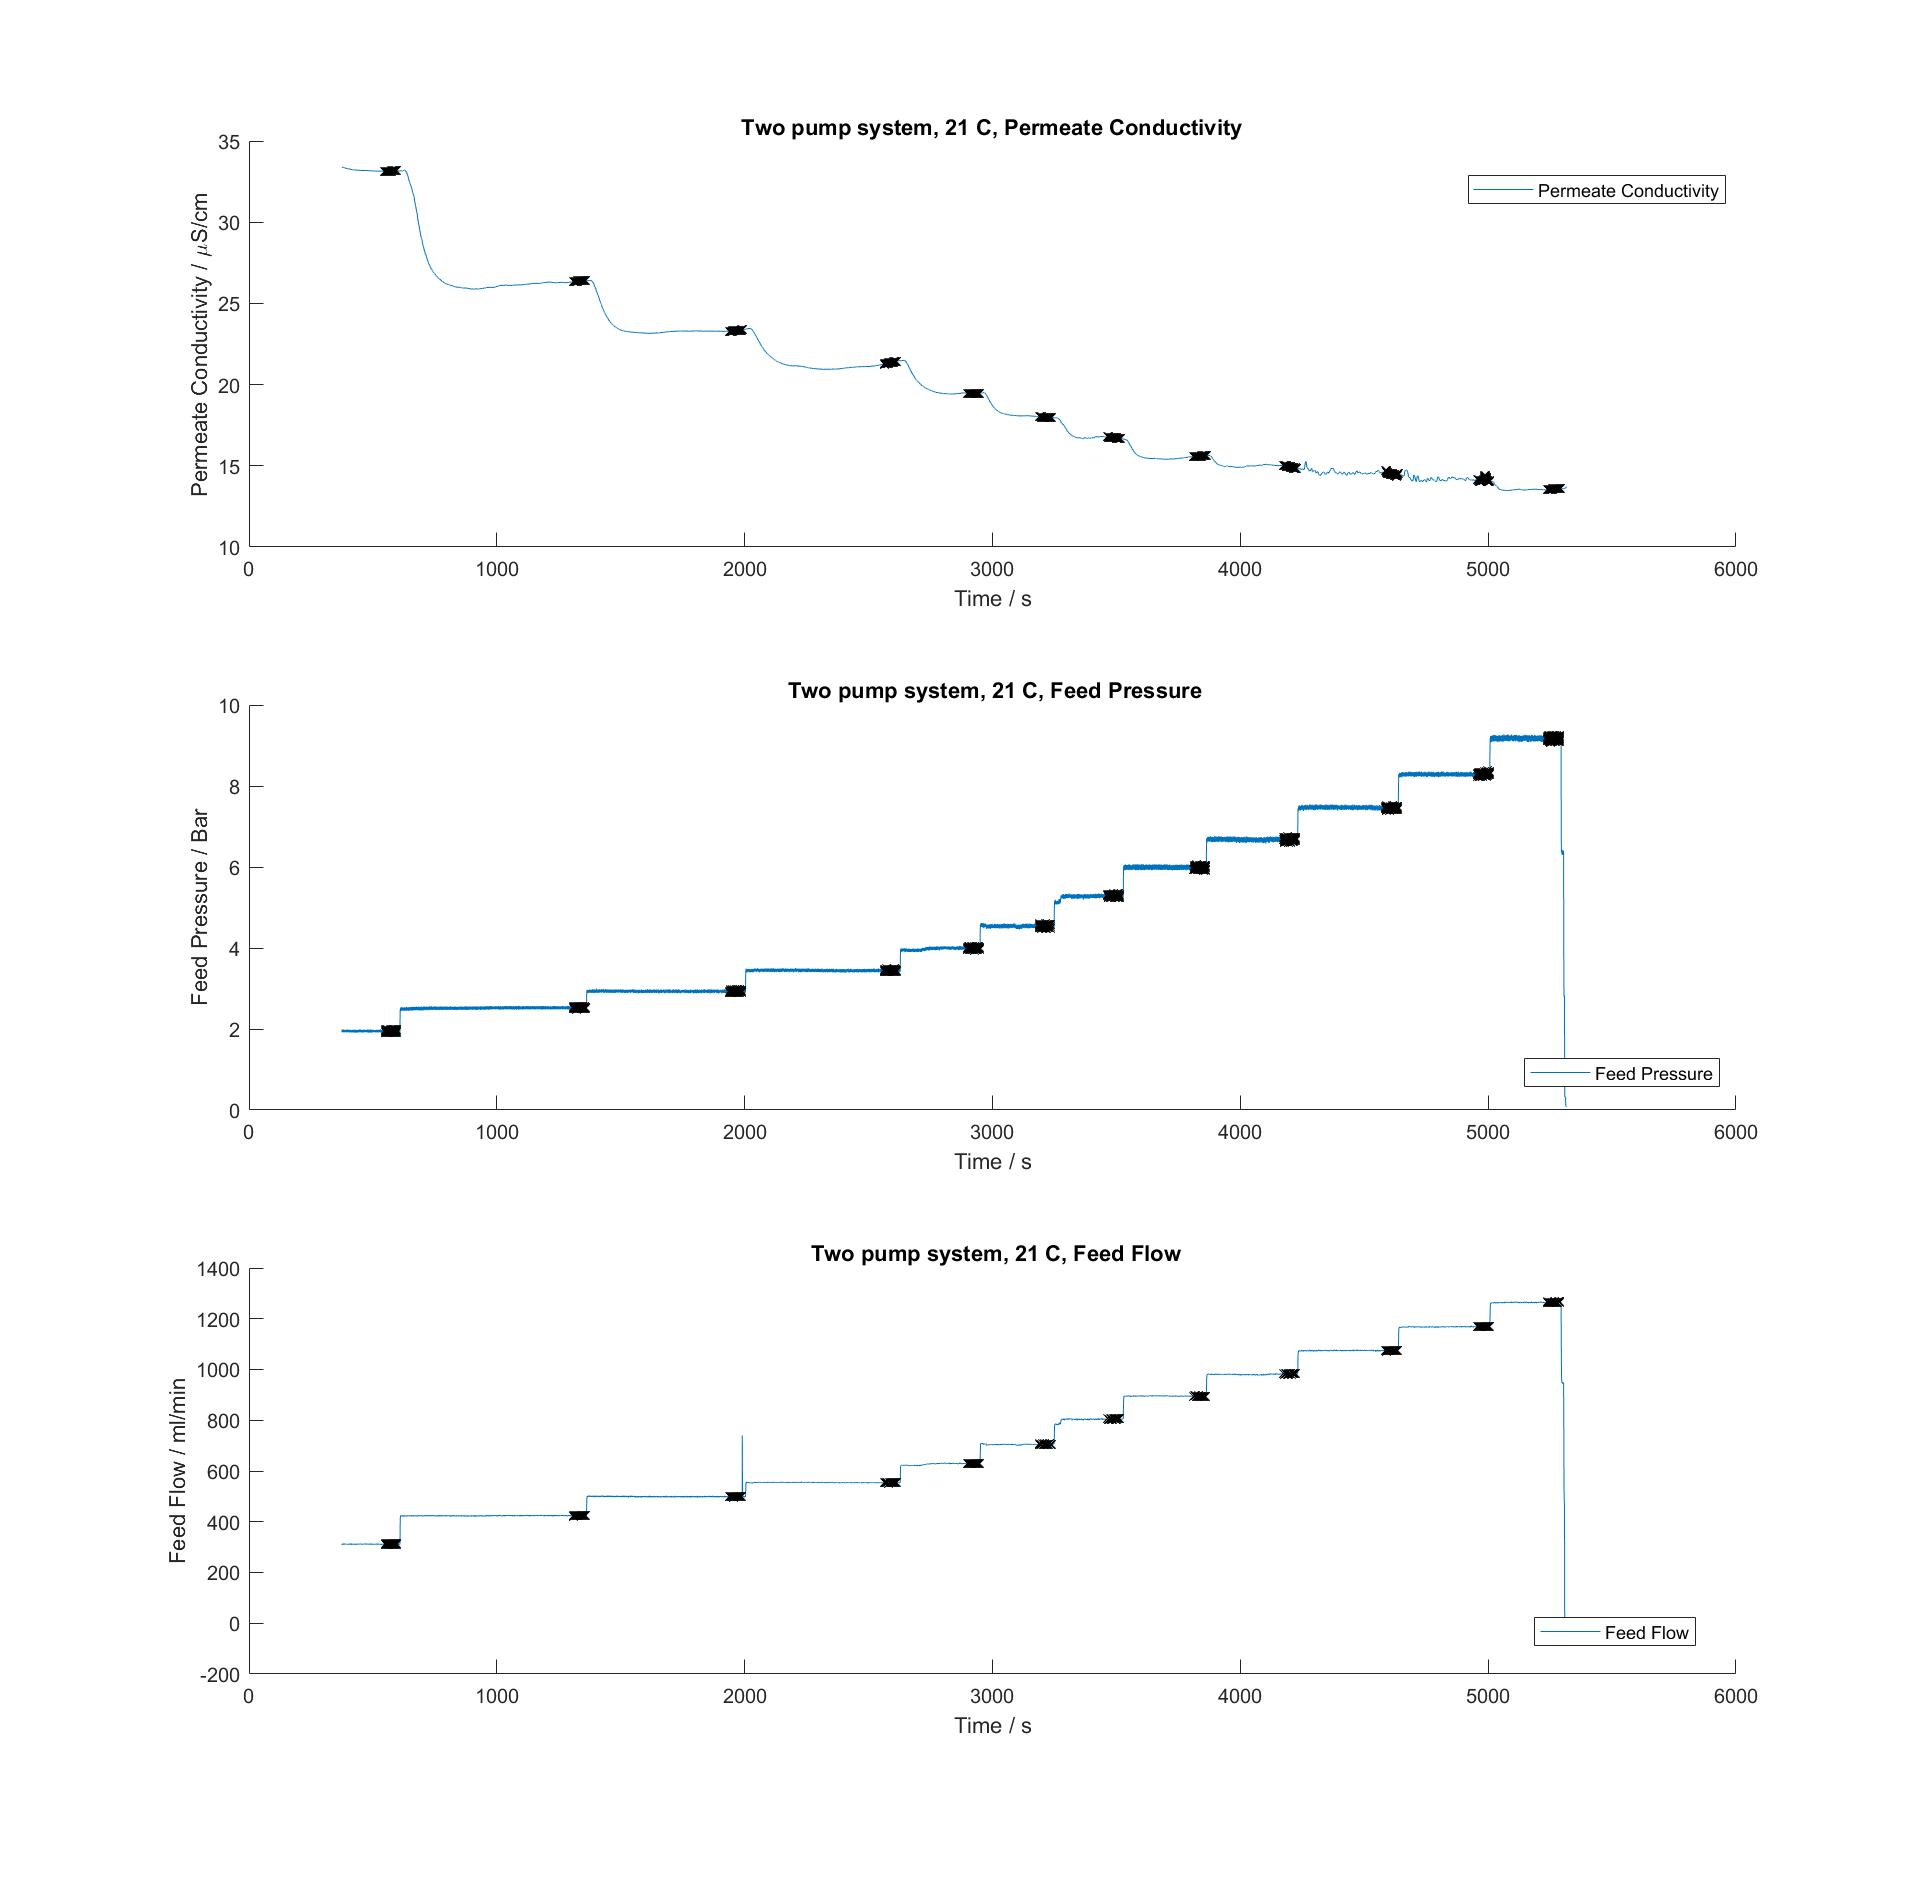
\includegraphics[width=1.1\textwidth]{FeedPumpIncrease21}
    \caption{Connections Pressure sensors}
    \label{fig:PressConn}
\end{figure}


\begin{figure}[H]
    \centering
    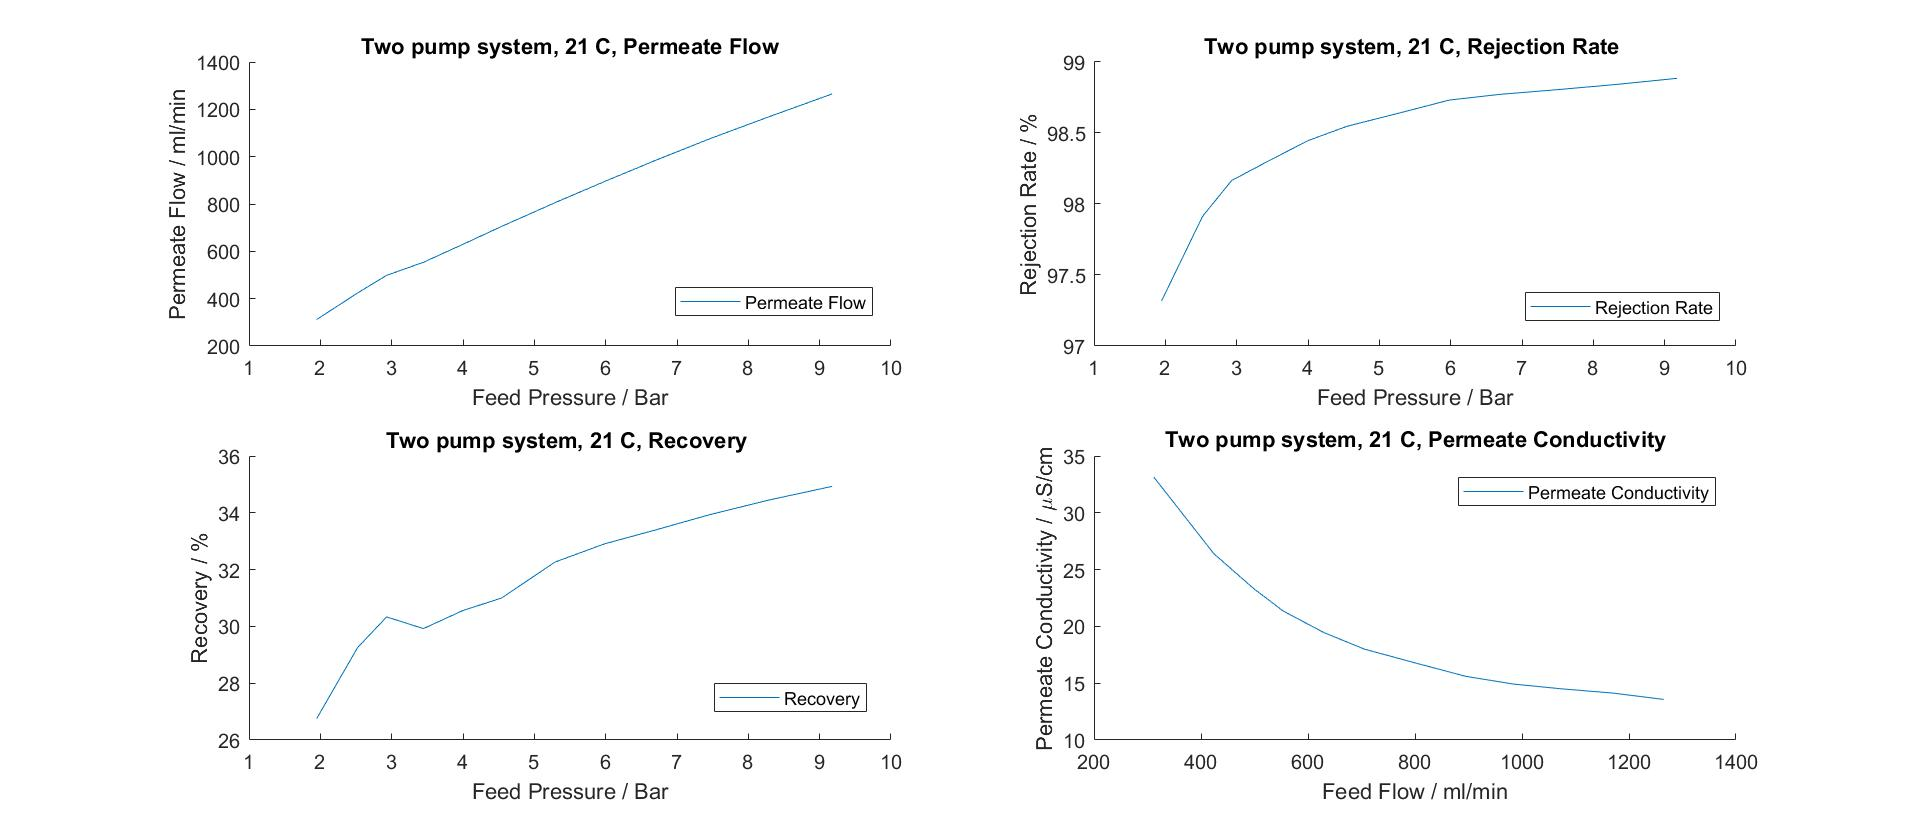
\includegraphics[width=1.1\textwidth]{FeedPumpIncrease21Key}
    \caption{Connections Pressure sensors}
    \label{fig:PressConn}
\end{figure}

30


\begin{figure}[H]
    \centering
    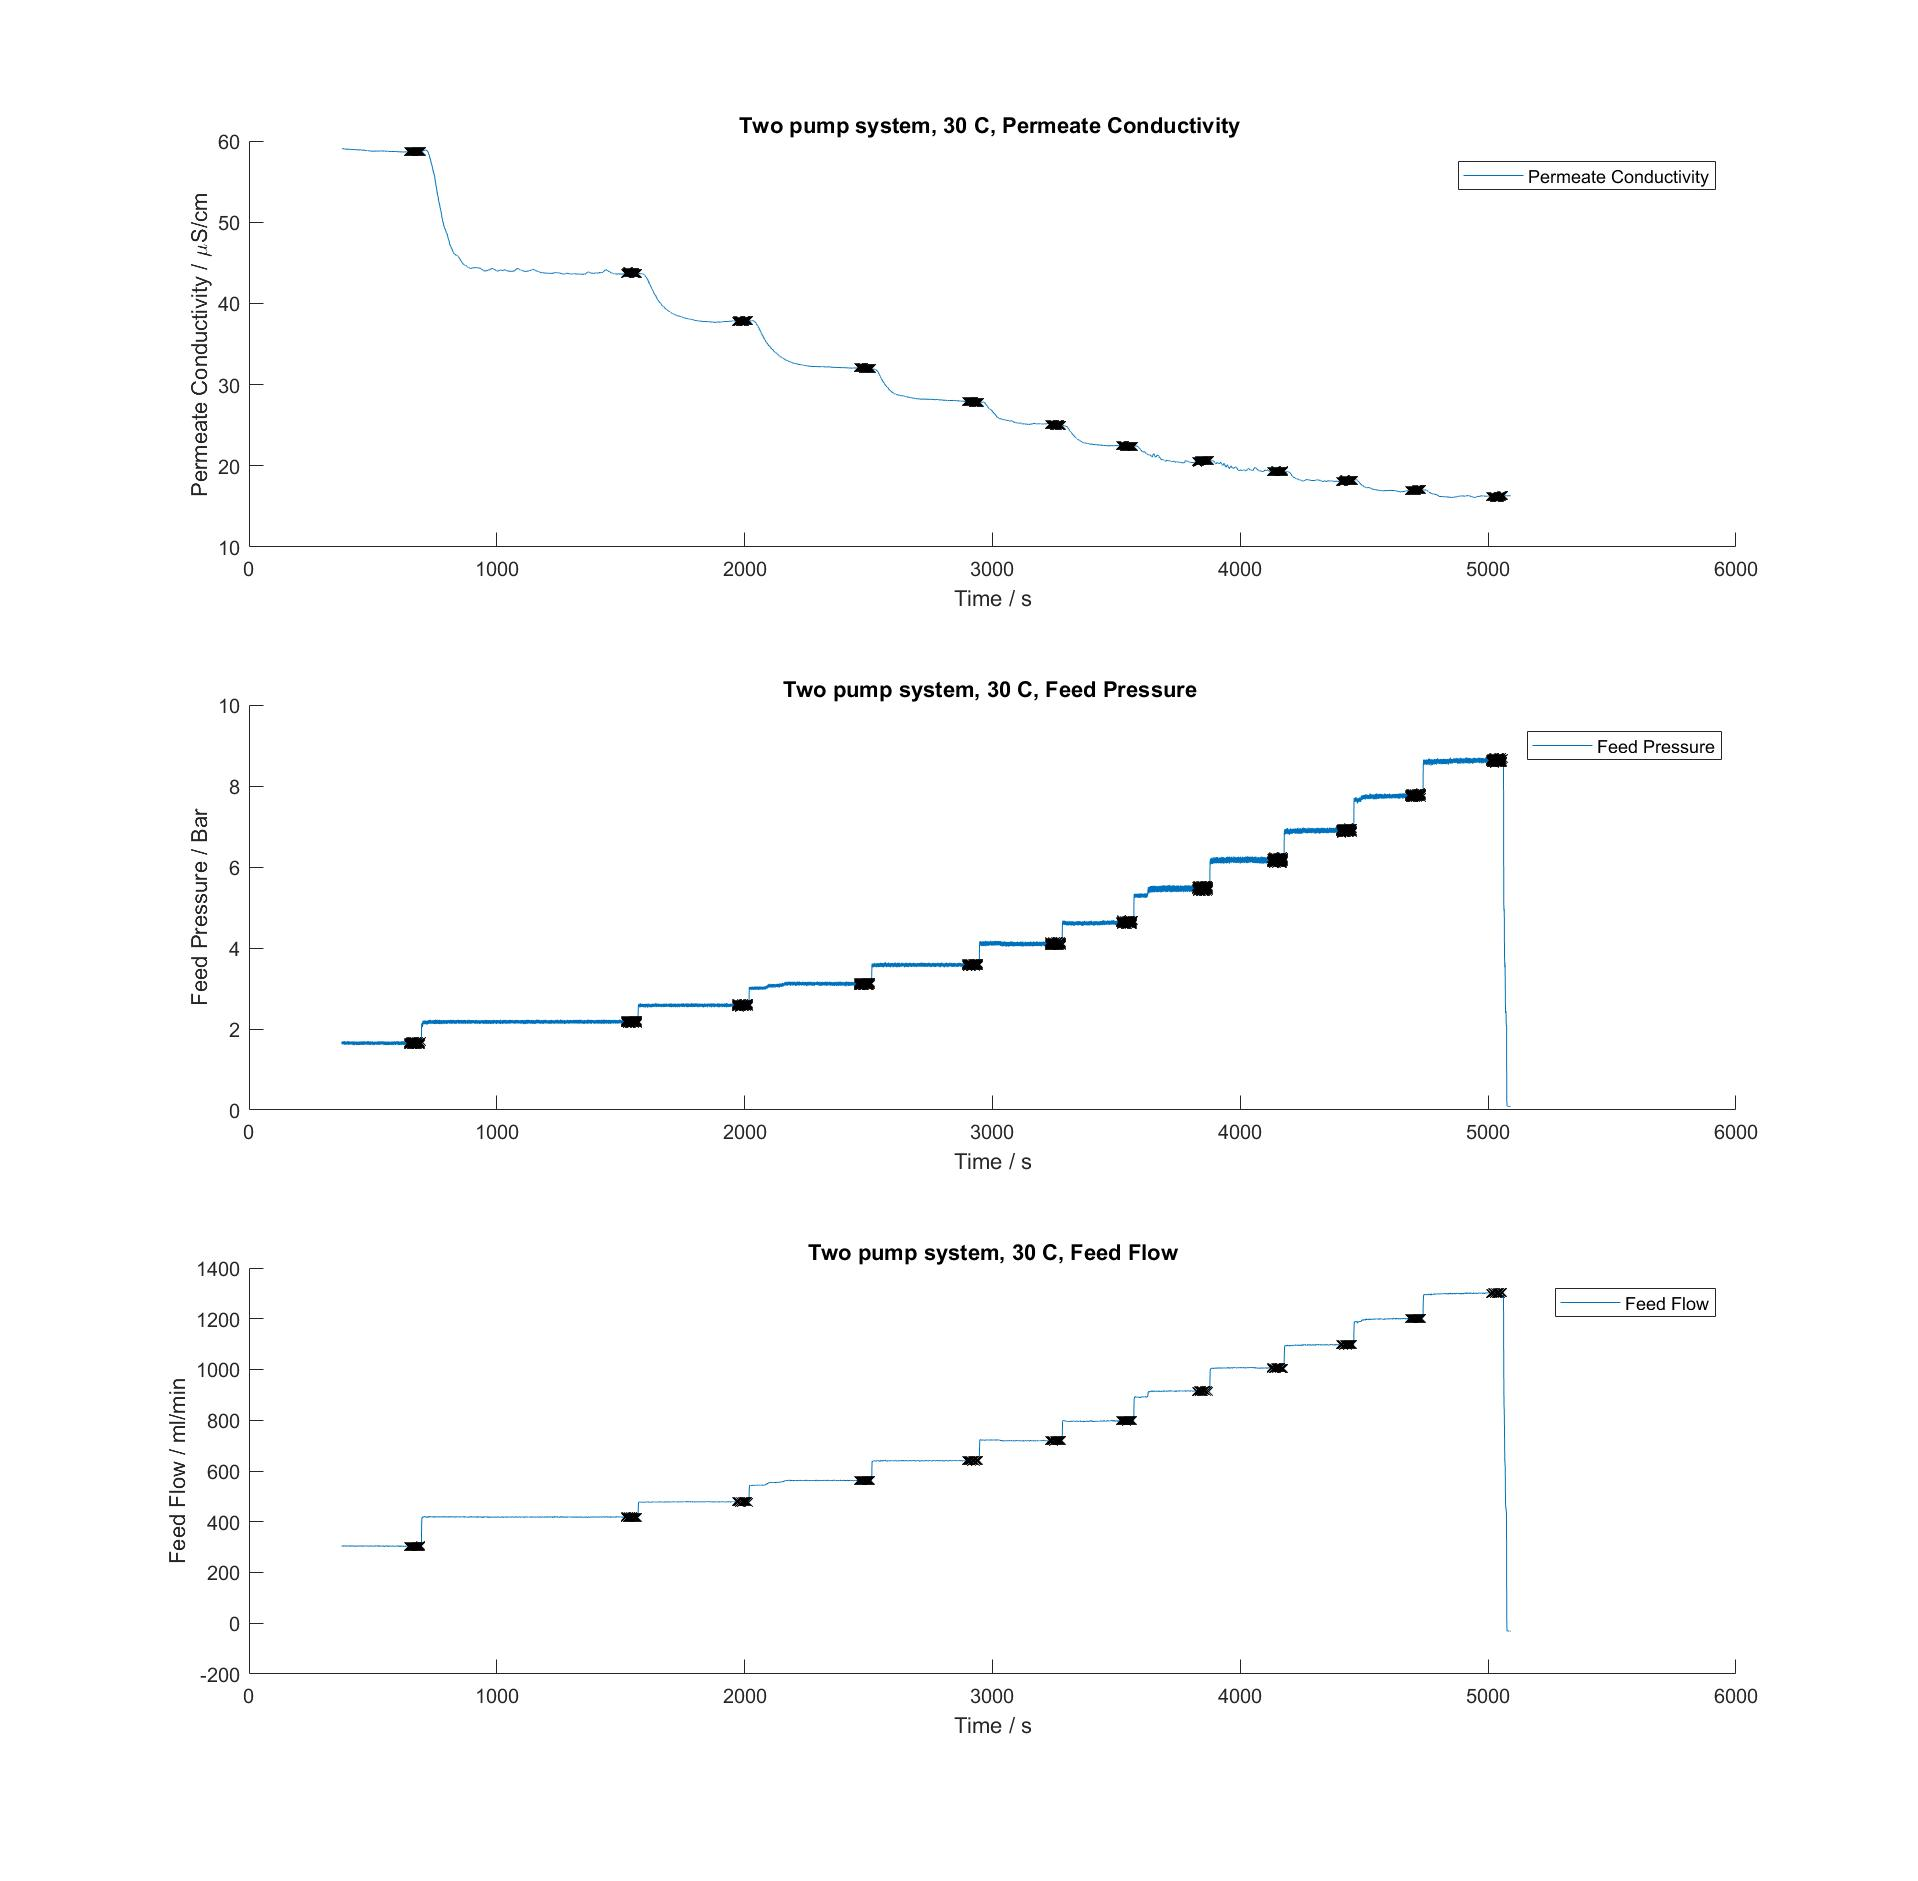
\includegraphics[width=1.1\textwidth]{FeedPumpIncrease30}
    \caption{Connections Pressure sensors}
    \label{fig:PressConn}
\end{figure}


\begin{figure}[H]
    \centering
    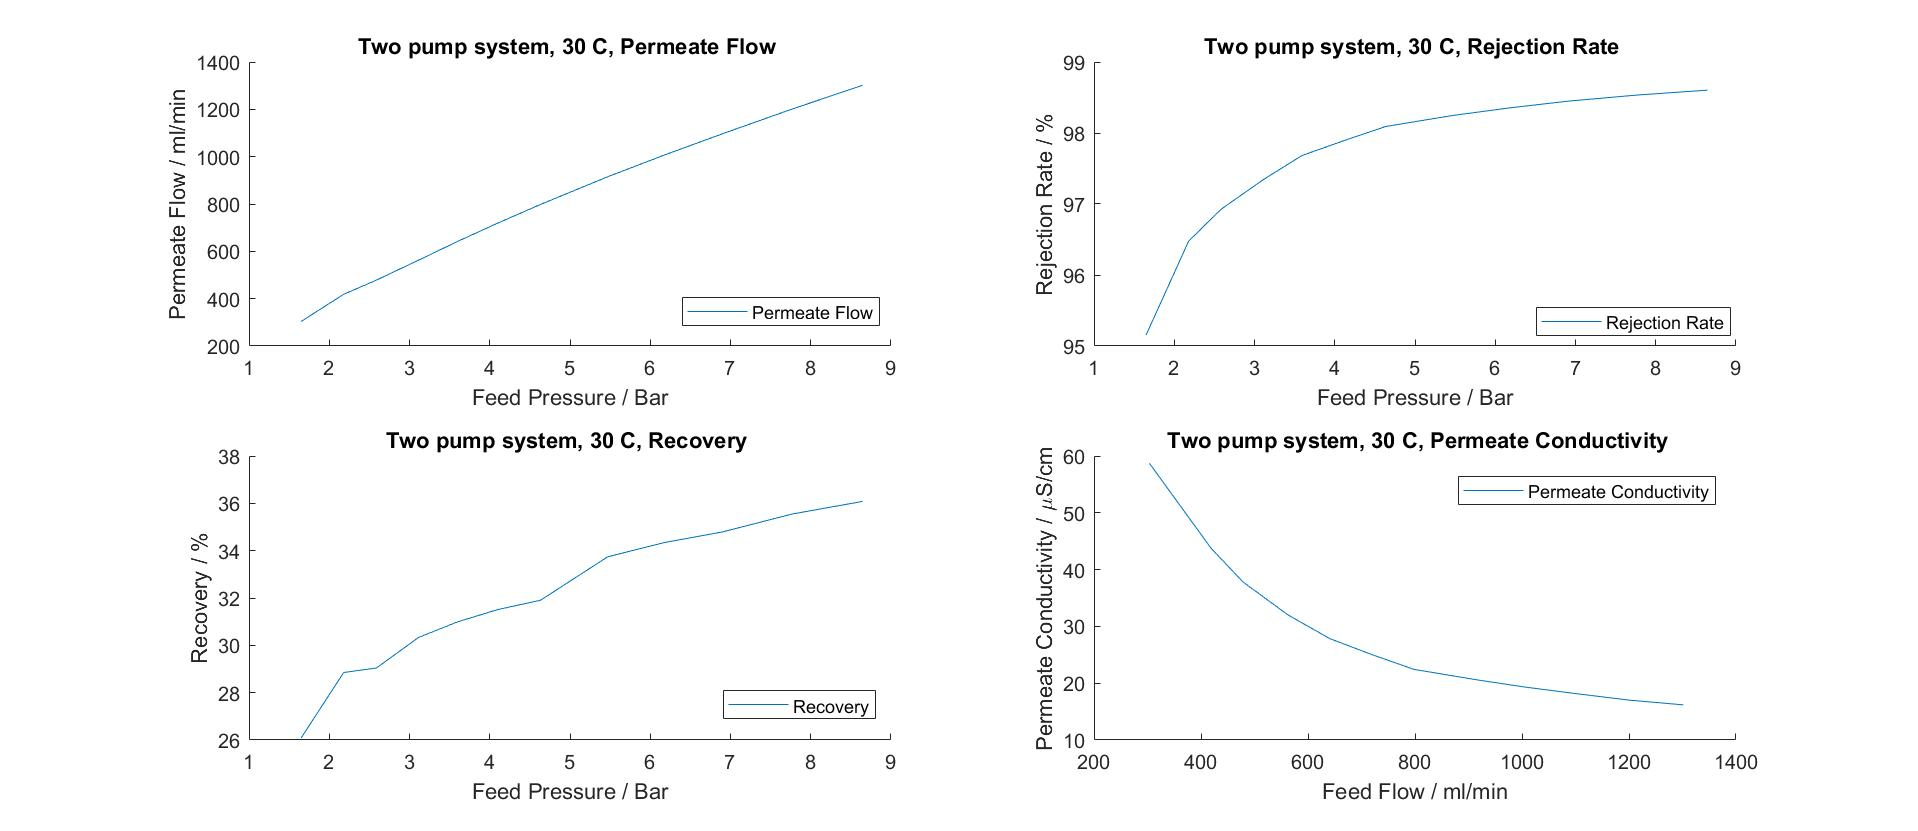
\includegraphics[width=1.1\textwidth]{FeedPumpIncrease30Key}
    \caption{Connections Pressure sensors}
    \label{fig:PressConn}
\end{figure}

40


\begin{figure}[H]
    \centering
    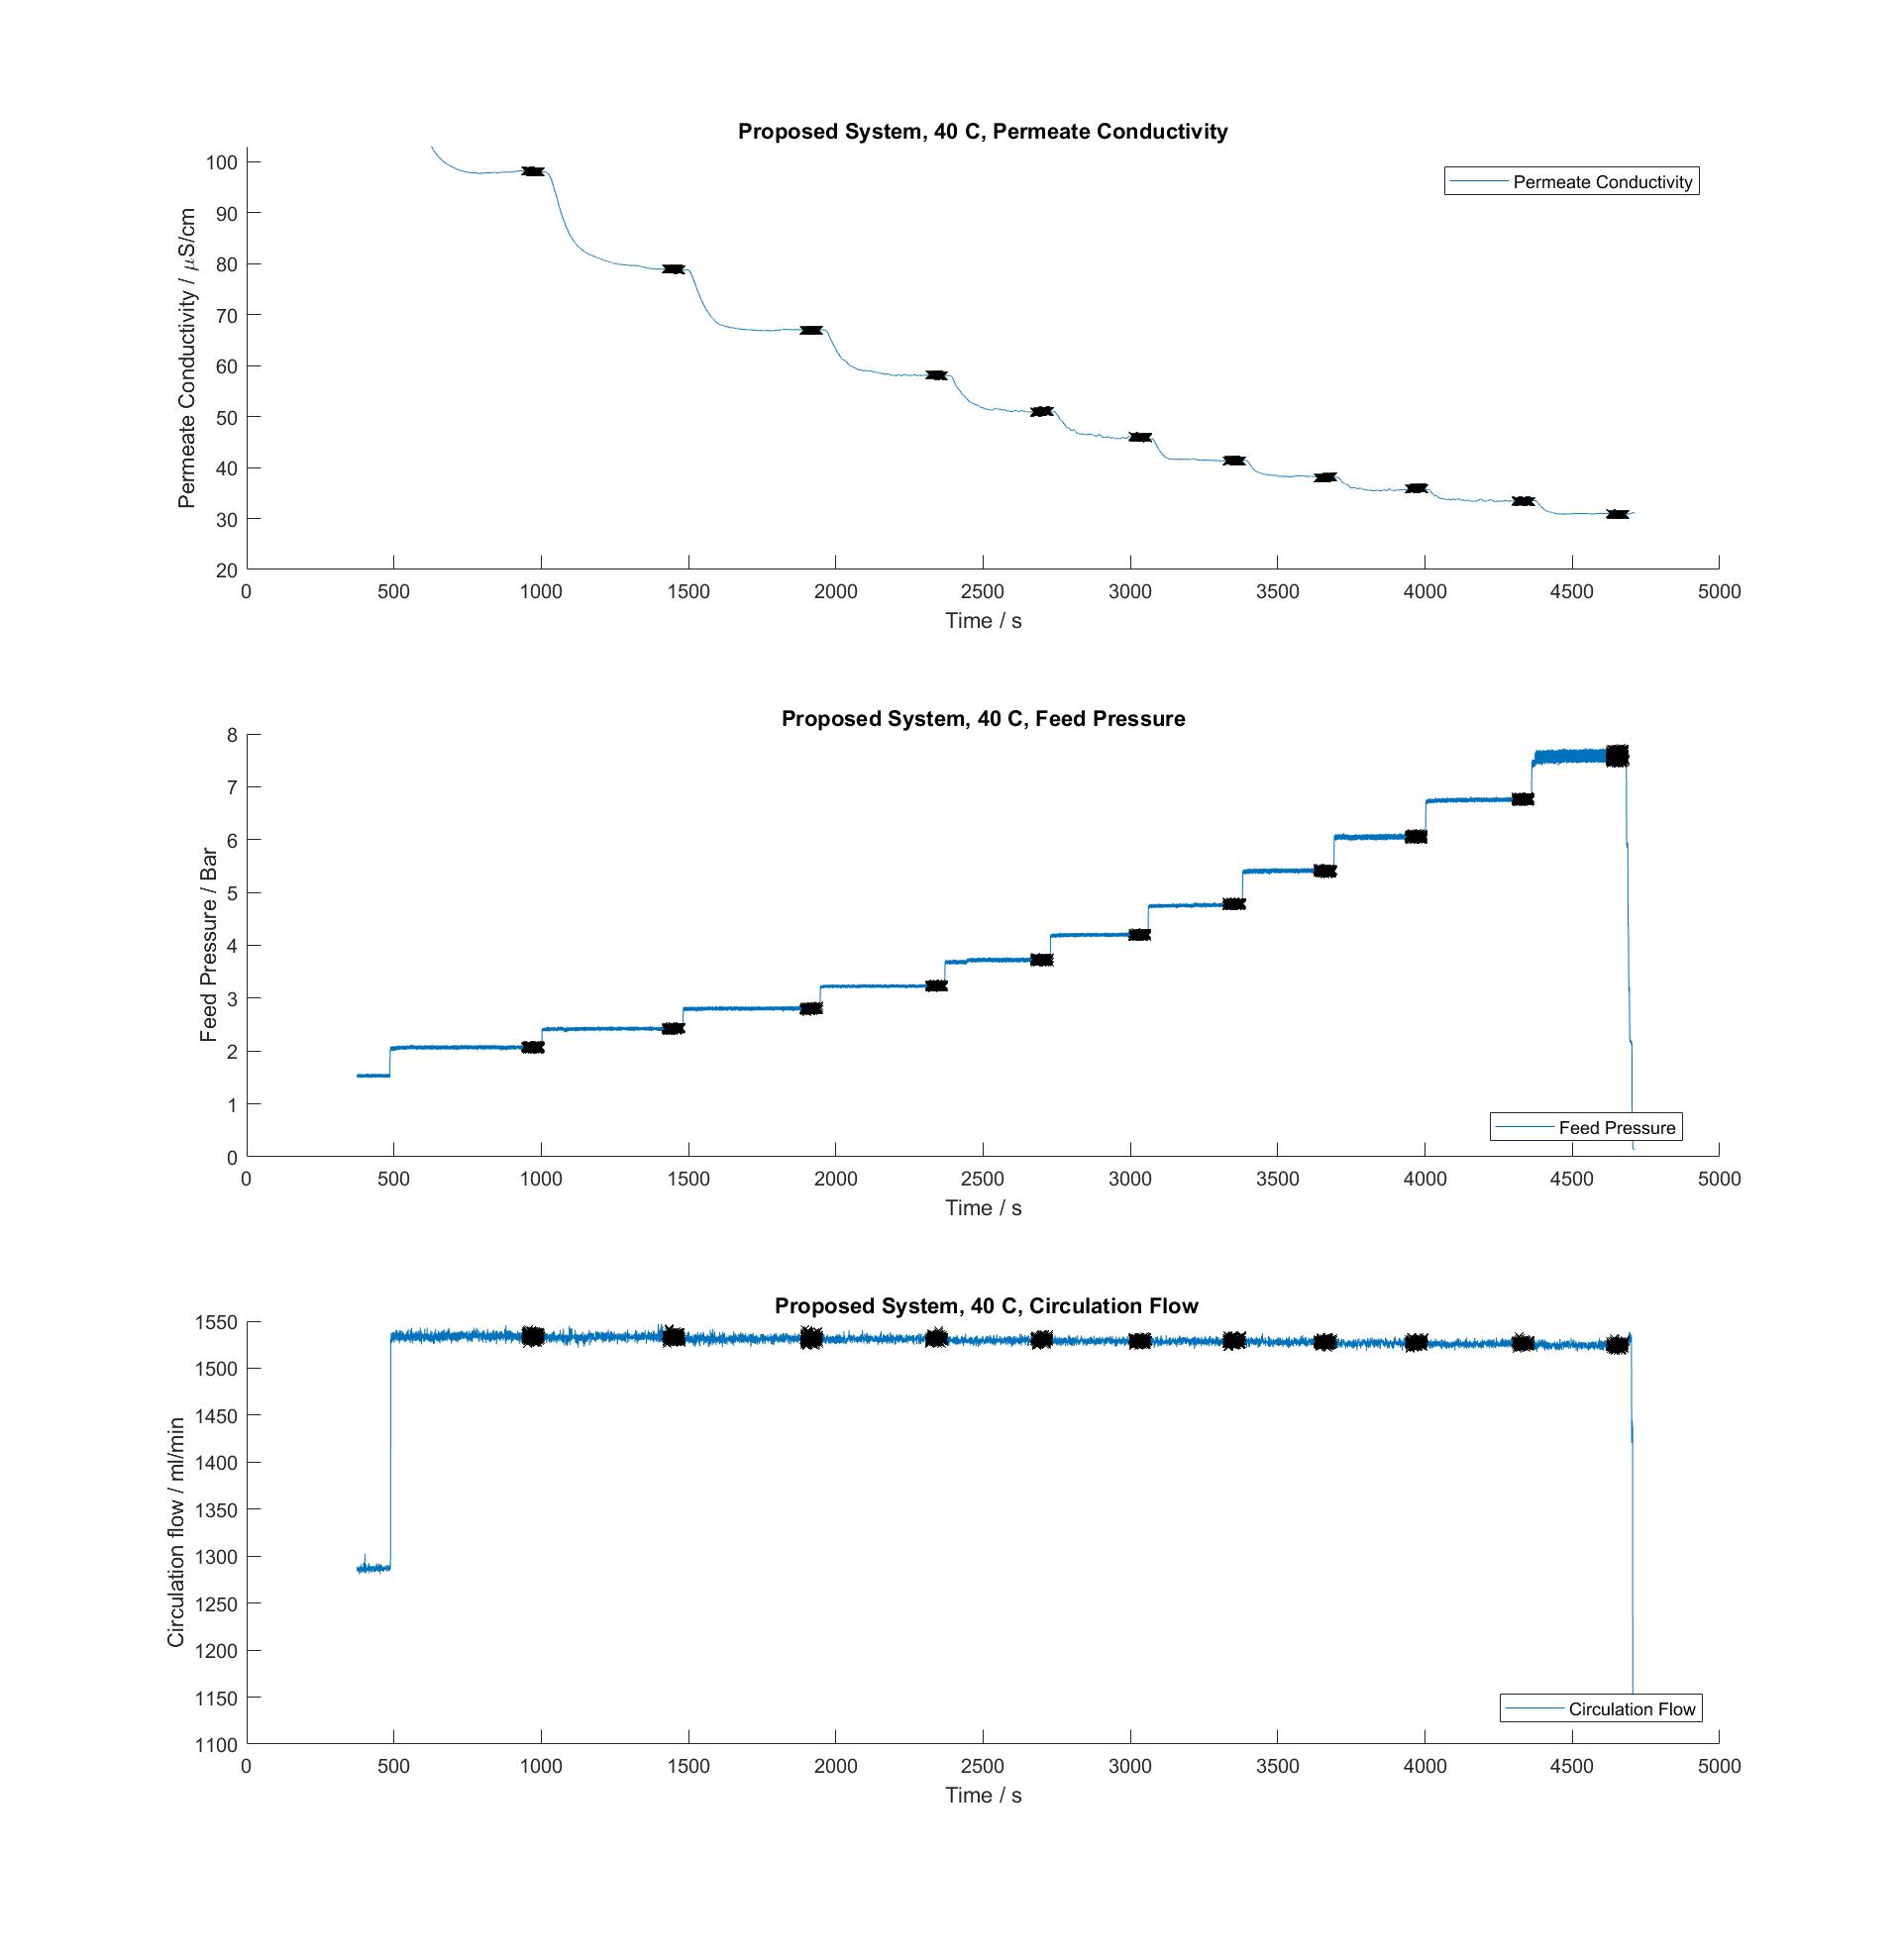
\includegraphics[width=1.1\textwidth]{FeedPumpIncrease40}
    \caption{Connections Pressure sensors}
    \label{fig:PressConn}
\end{figure}


\begin{figure}[H]
    \centering
    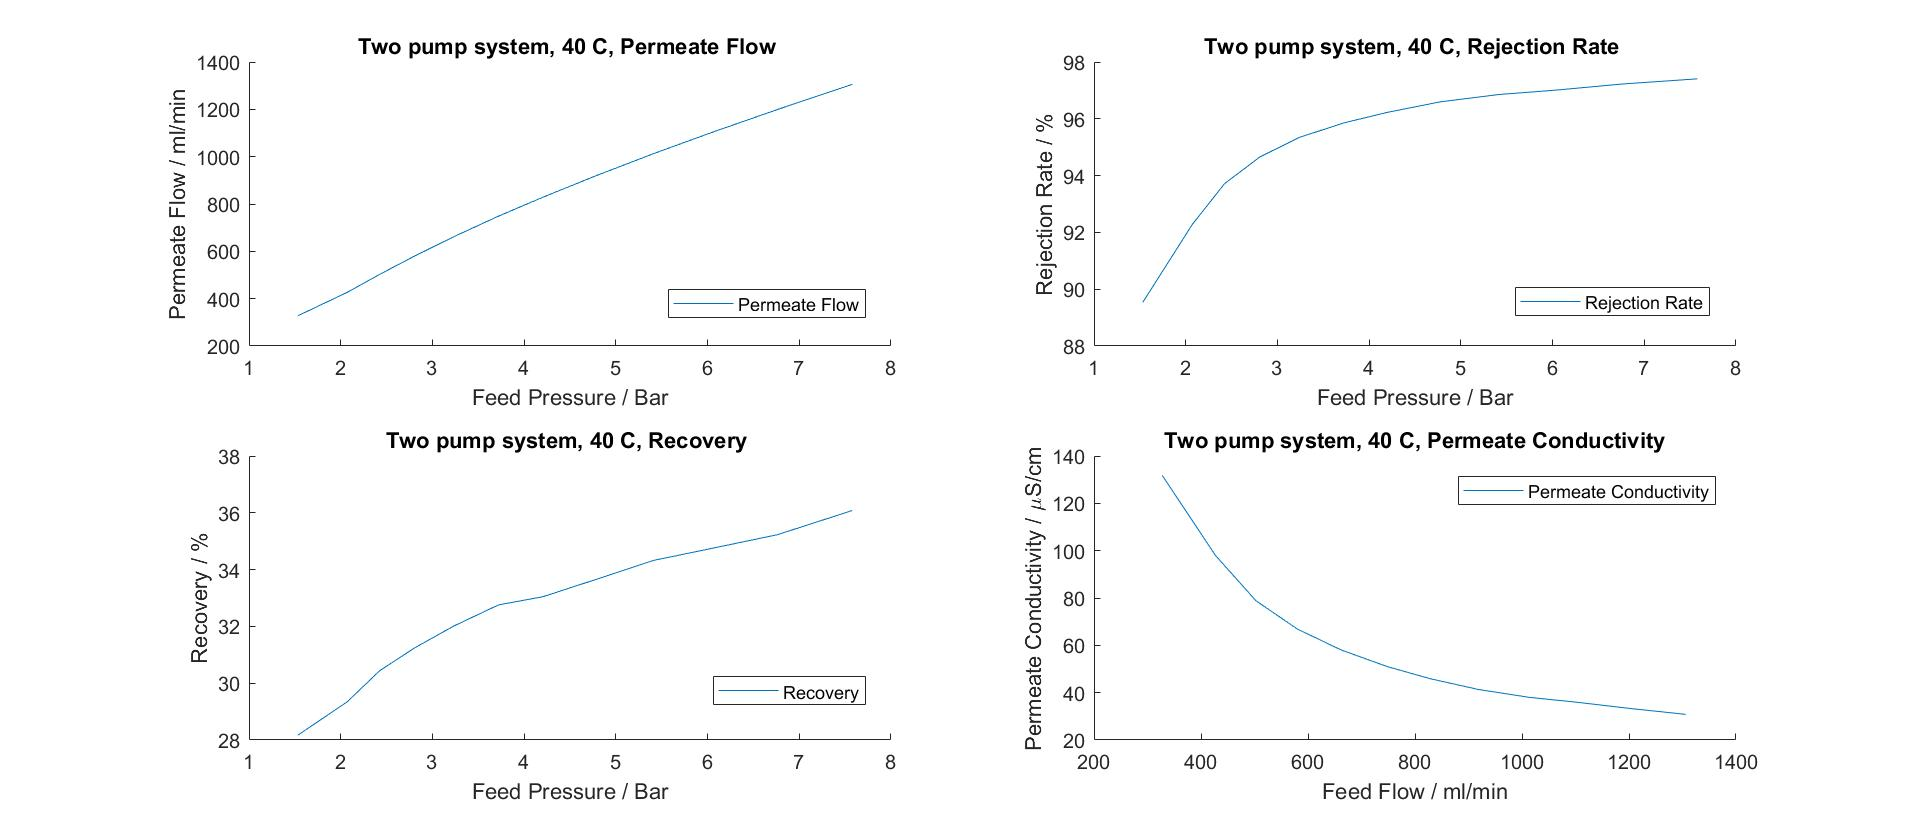
\includegraphics[width=1.1\textwidth]{FeedPumpIncrease40Key}
    \caption{Connections Pressure sensors}
    \label{fig:PressConn}
\end{figure}

Recovery Increase

\begin{figure}[H]
    \centering
    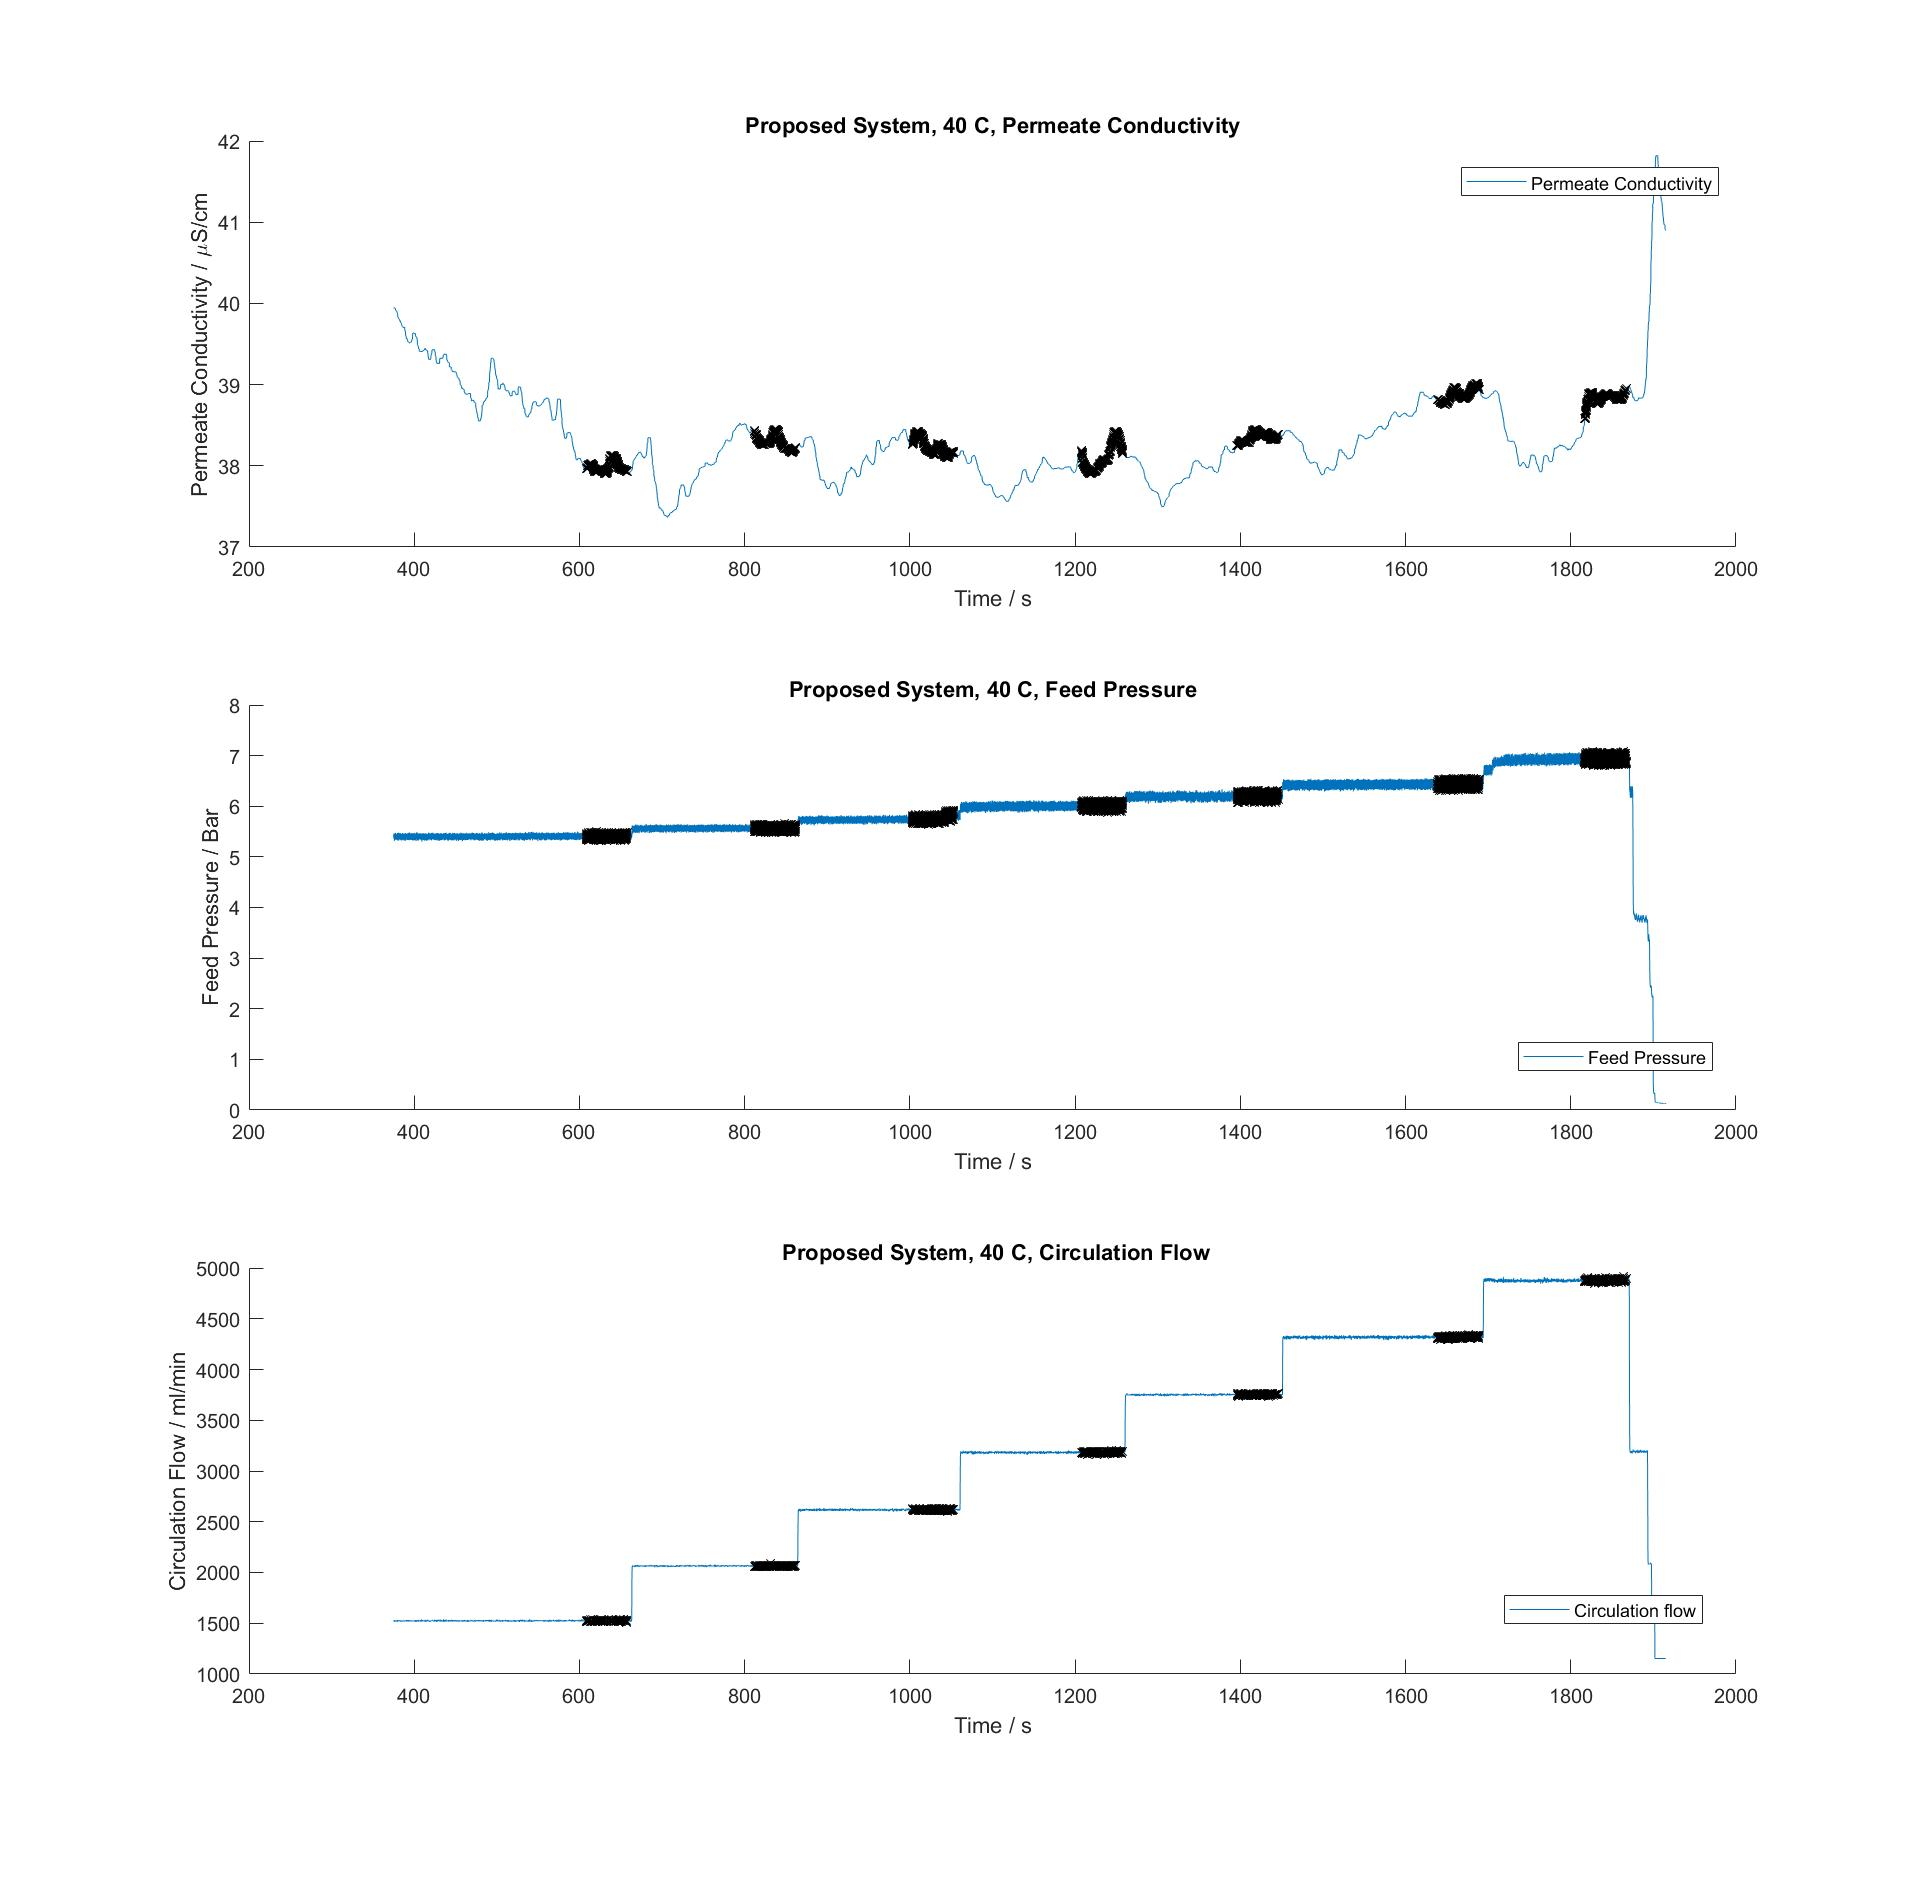
\includegraphics[width=1.1\textwidth]{RecIncrease40}
    \caption{Connections Pressure sensors}
    \label{fig:PressConn}
\end{figure}

\begin{figure}[H]
    \centering
    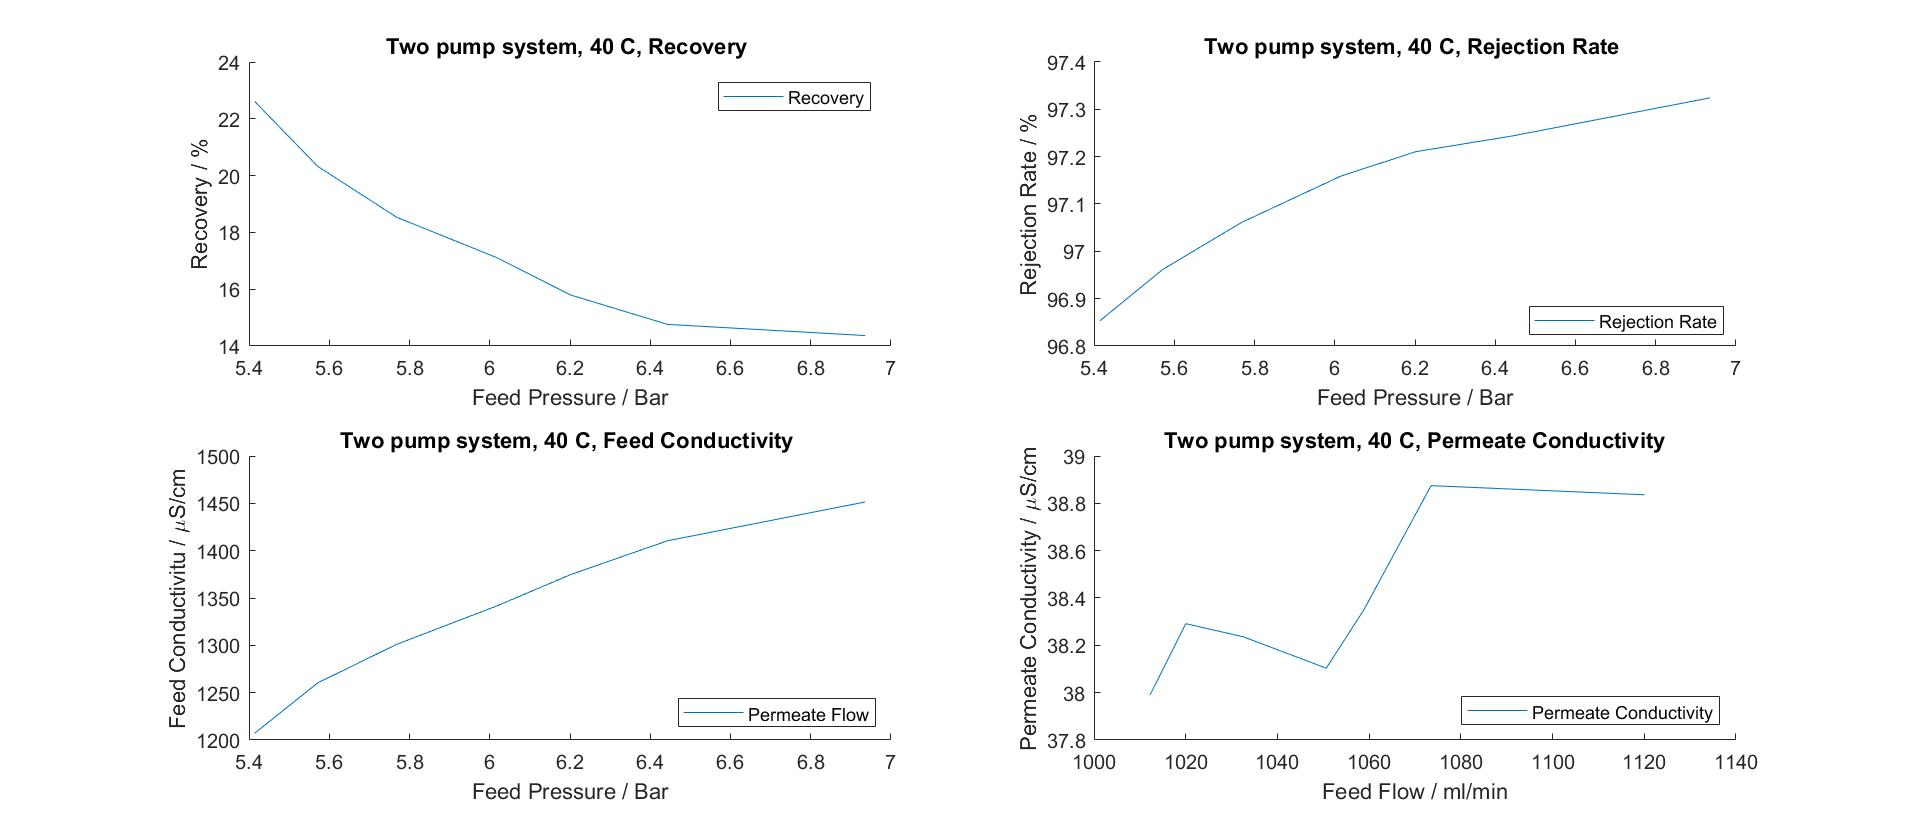
\includegraphics[width=1.1\textwidth]{RecIncrease40Key}
    \caption{Connections Pressure sensors}
    \label{fig:PressConn}
\end{figure}








\section{Modeling}
A physical model of the membrane were made and the given results can be seen in: 

\section{Implementation Test Rig}


\subsection{Connections}
In Figure (\ref{fig:PressConn}-\ref{fig:PumpConn}) all connections in the test rig is displayed.


\begin{figure}[h]
    \centering
    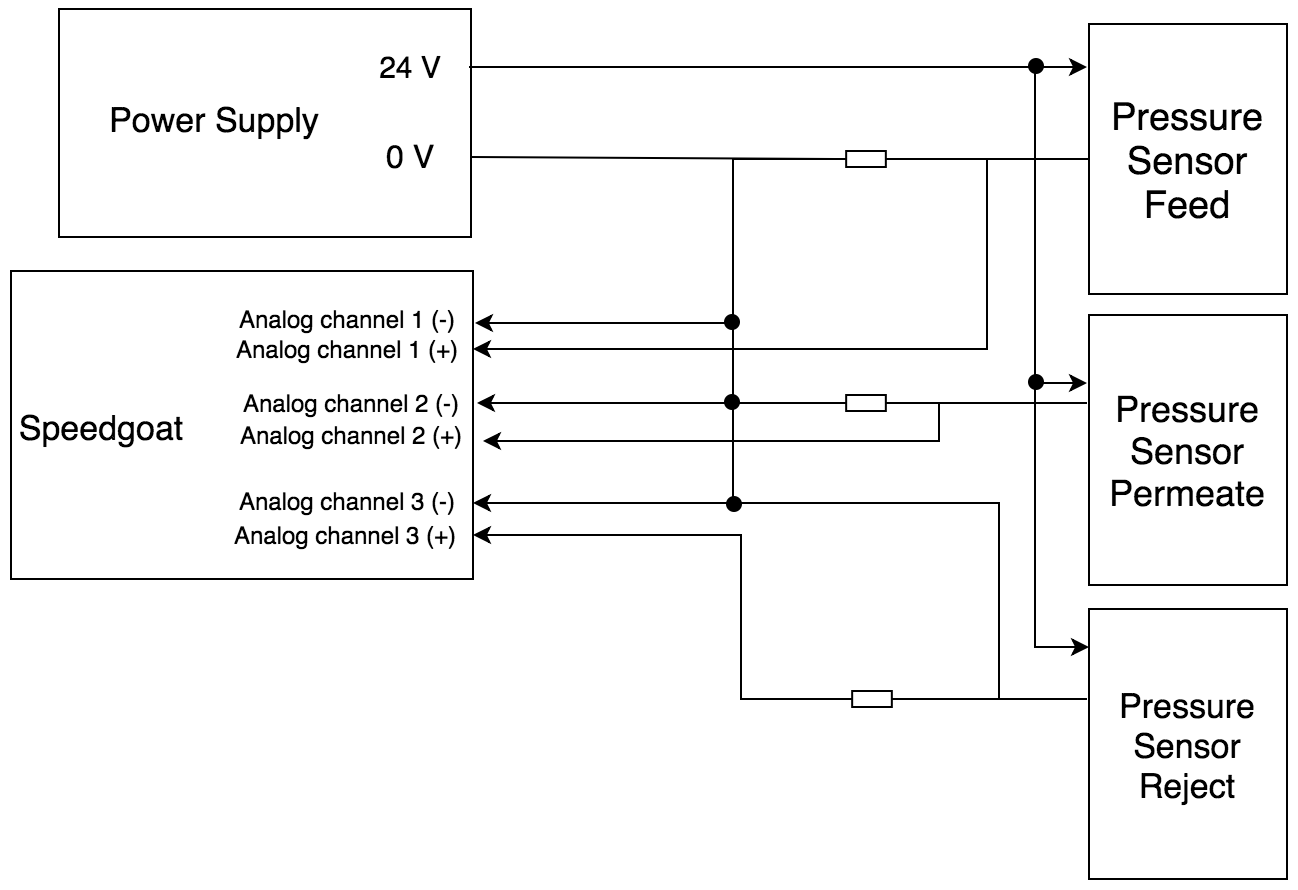
\includegraphics[width=0.7\textwidth]{PressConn}
    \caption{Connections Pressure sensors}
    \label{fig:PressConn}
\end{figure}

\begin{figure}[h]
    \centering
    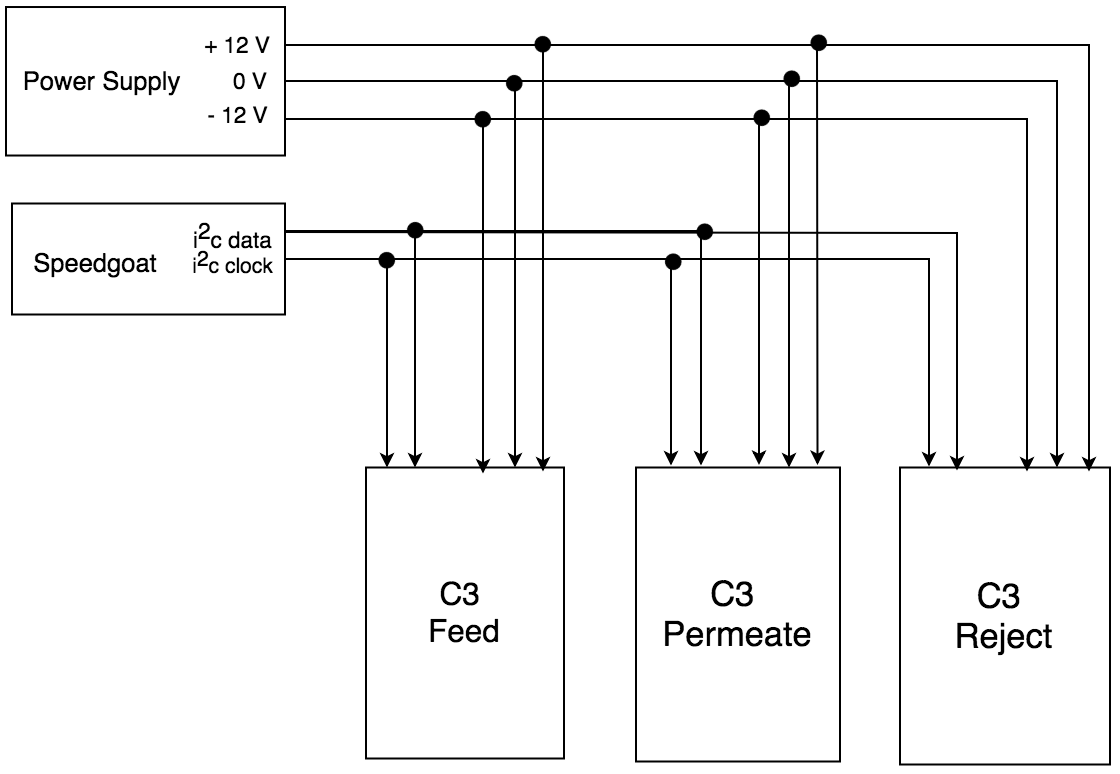
\includegraphics[width=0.7\textwidth]{C3Conn}
    \caption{Connections measurement blocks, C3}
    \label{fig:C3Conn}
\end{figure}

\begin{figure}[h]
    \centering
    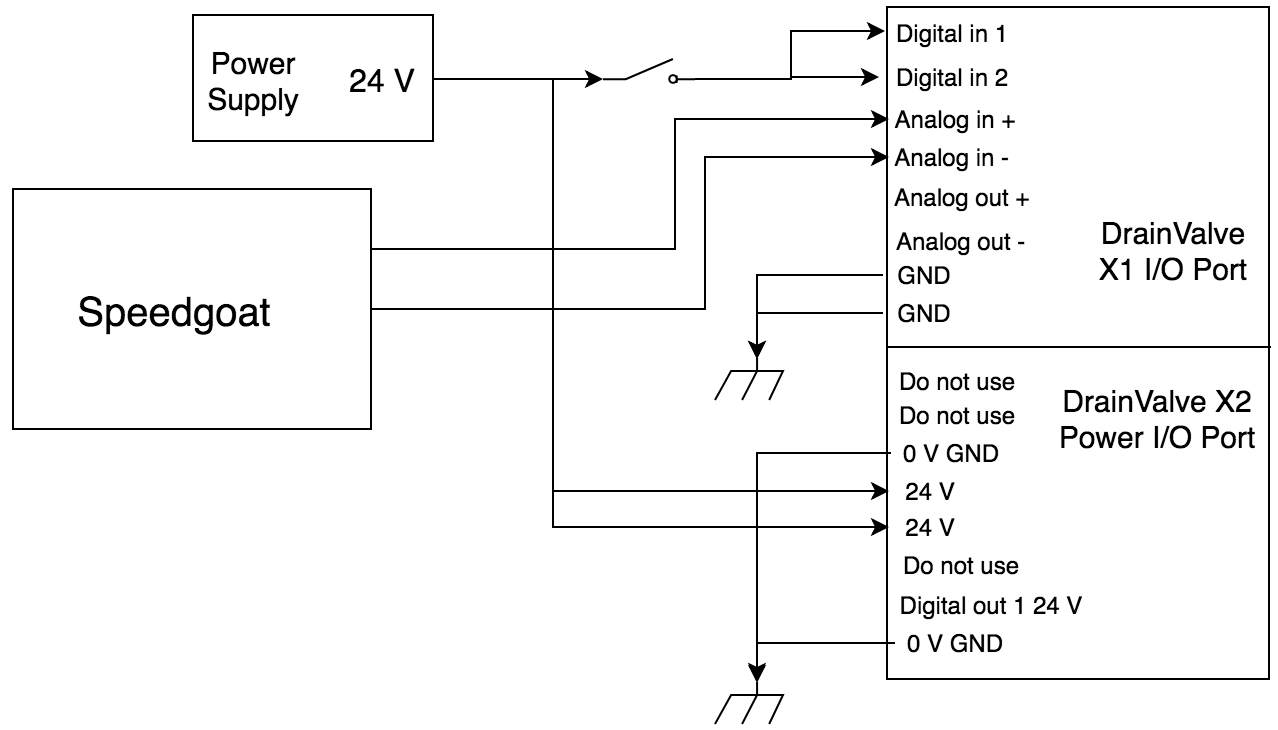
\includegraphics[width=0.7\textwidth]{ValveConn}
    \caption{Connections Drain Valve}
    \label{fig:ValveConn}
\end{figure}

\begin{figure}[h]
    \centering
    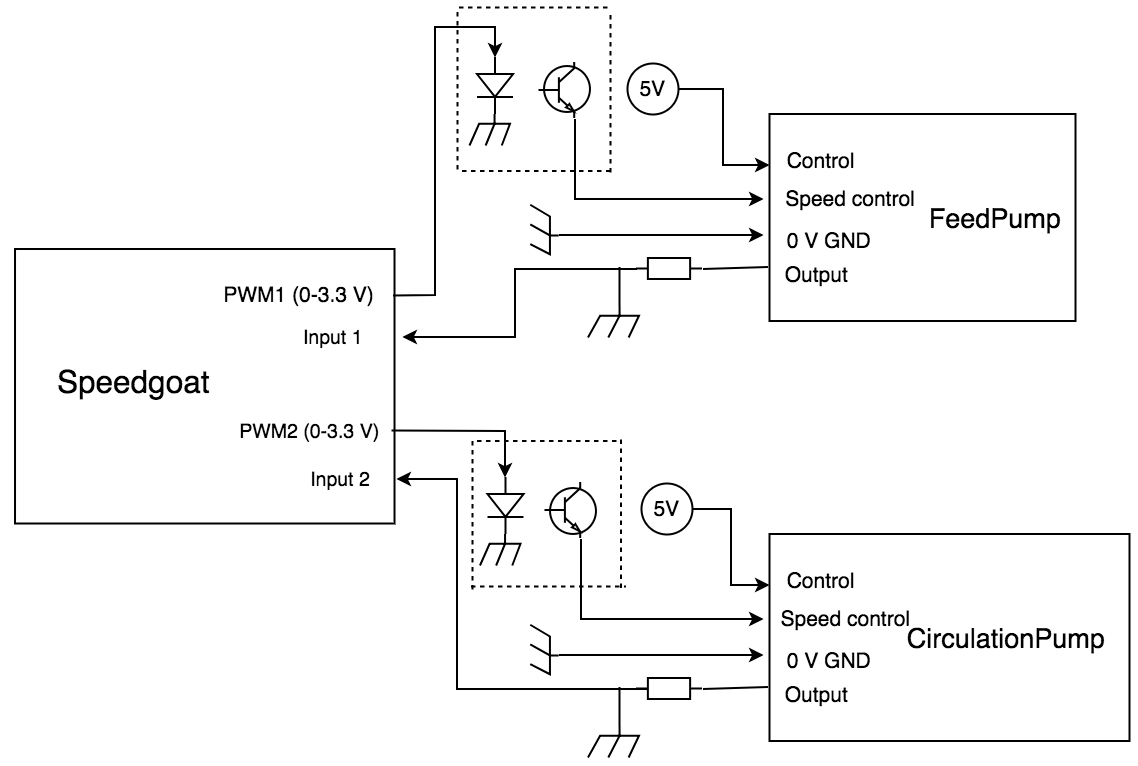
\includegraphics[width=0.7\textwidth]{PumpConn}
    \caption{Connections pumps}
    \label{fig:PumpConn}
\end{figure}


\section{Mapping}
\begin{figure}[h]
    \centering
    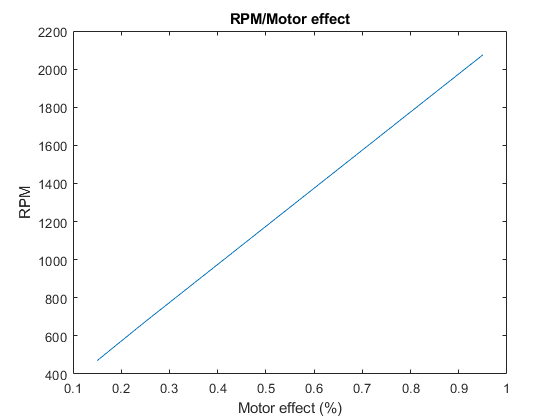
\includegraphics[width=0.7\textwidth]{RPM.png}
    \caption{RPM Pumps}
    \label{fig:RPM}
\end{figure}


\begin{figure}[h]
    \centering
    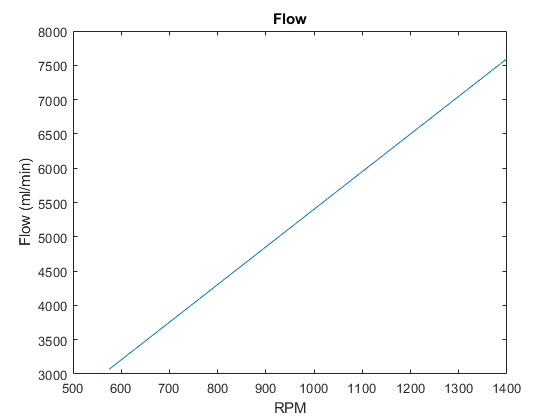
\includegraphics[width=0.7\textwidth]{Flow.png}
    \caption{Flowrate}
    \label{fig:Flowrate}
\end{figure}


\section{Design of control algorithms}

\begin{figure}[h]
    \centering
    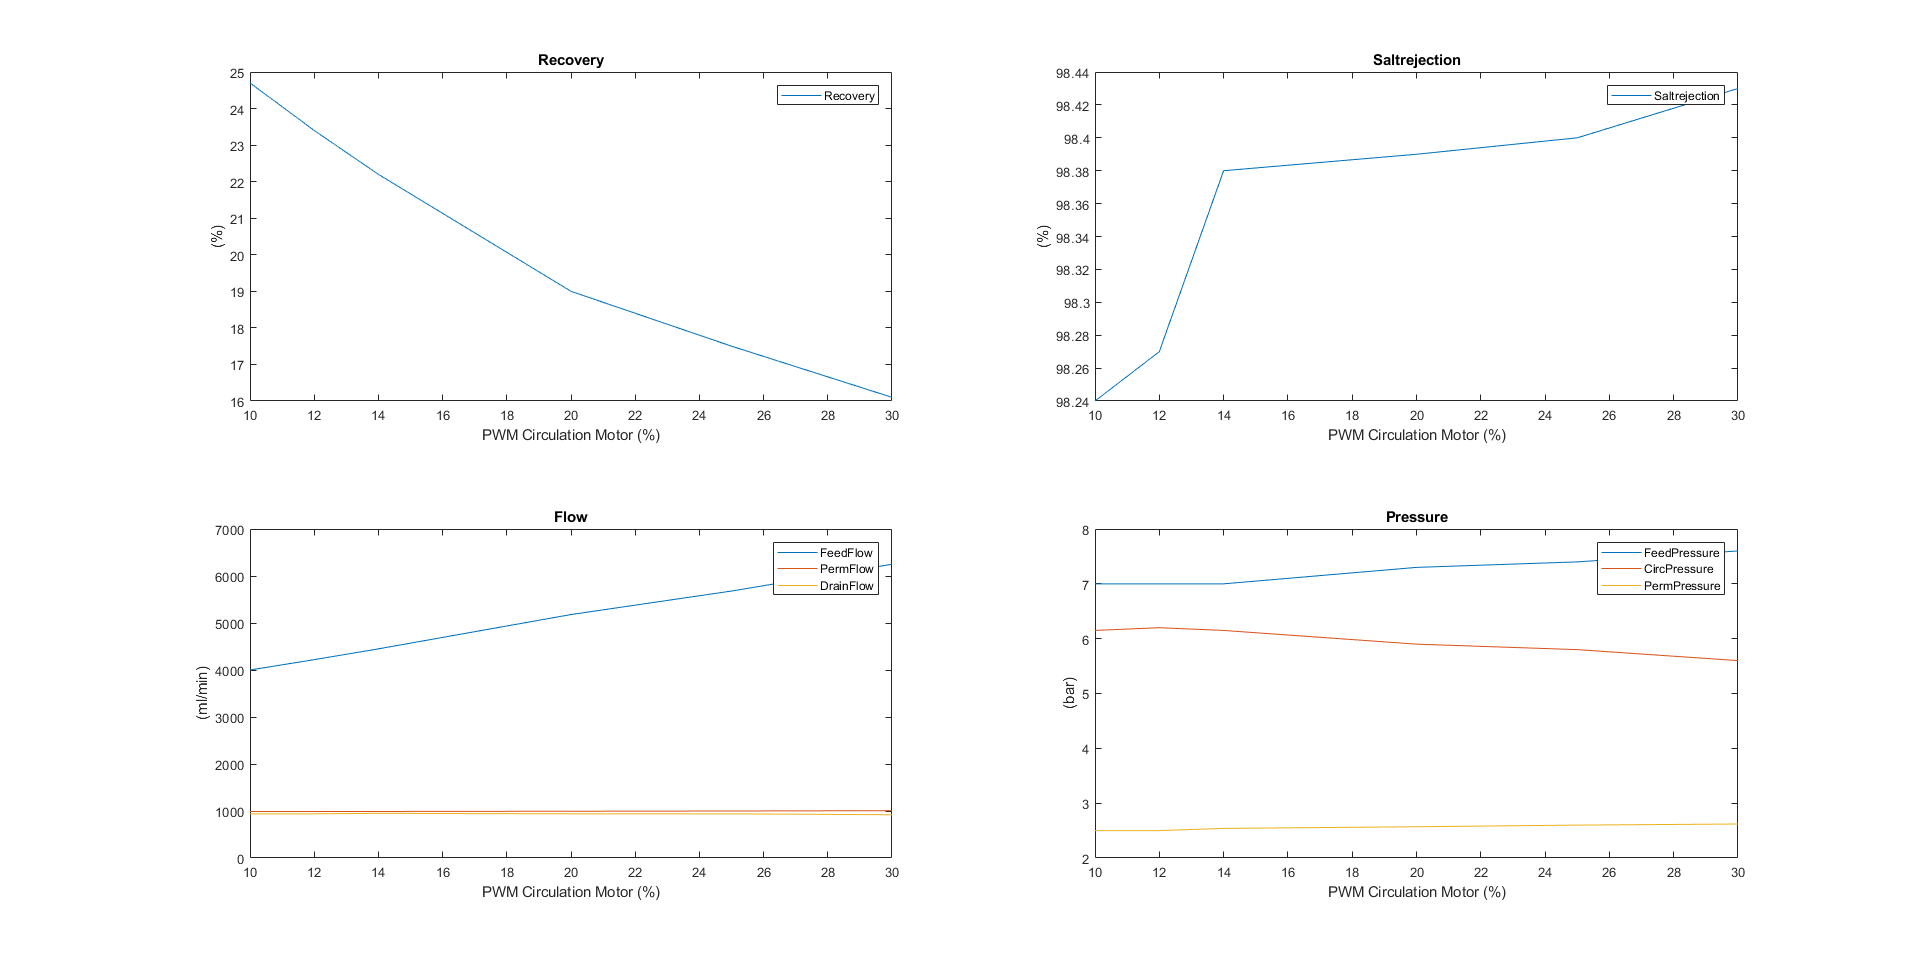
\includegraphics[width=1.65\textwidth, angle = 270]{PreTestReg1.png}
    \caption{Tests with recycle pump as changing parameter}
    \label{fig:PreTestReg1}
\end{figure}

\begin{figure}[h]
    \centering 
    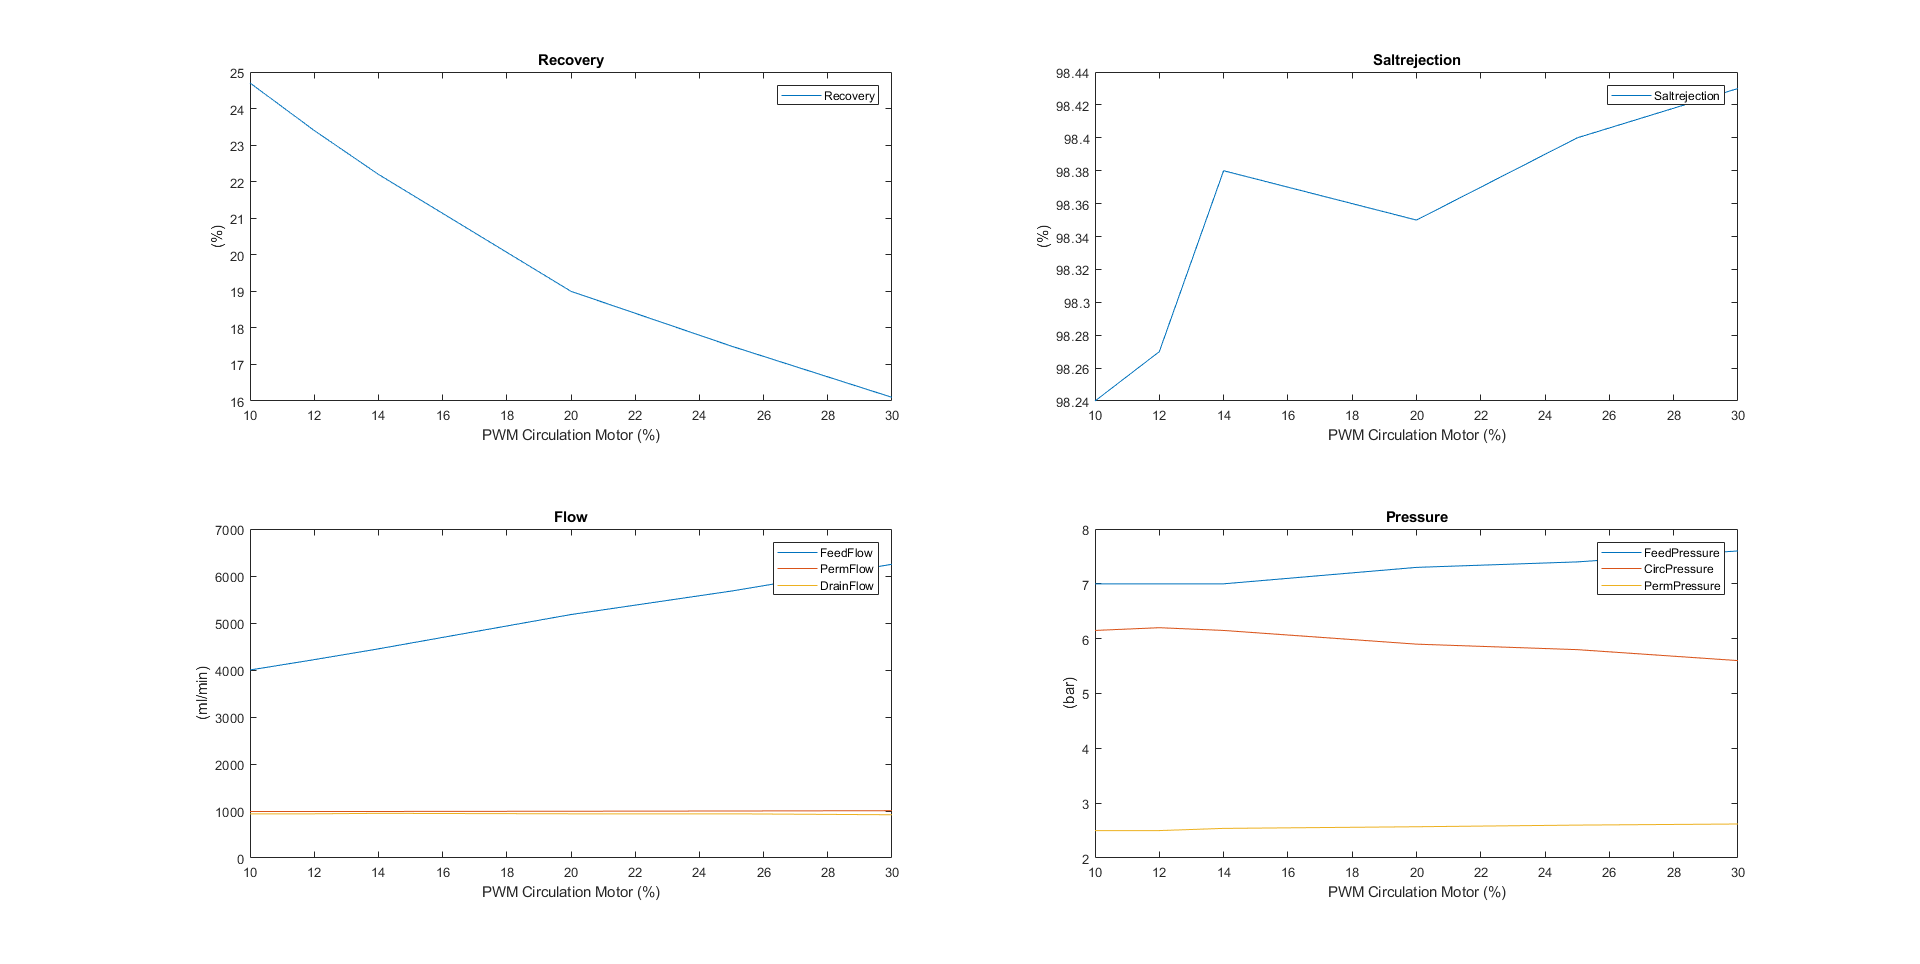
\includegraphics[width=1.65\textwidth, angle=270]{PreTestReg3.png}
    \caption{Tests with inlet pump as changing parameter}
    \label{fig:PreTestReg3}
\end{figure}





FIGURES AND PLOTS FROM SIMSCAPE


\section{Control simulations}




\section{Improvements}
